% Williams Physics Thesis template
% Patterned after the work of Cole Meisenhelder '15
% Commented by Prof. Charlie Doret, 12/2016
% Uploaded to Overleaf by Dr. Kevin Flaherty, 5/2021

\documentclass[12pt, oneside]{book} 



% The \usepackage{} command will import predefined fonts, symbols, environments, etc.  For example, the ams packages below come from the American Mathematical Society and include all kinds of useful math symbols like integrals
\usepackage{amscd}
\usepackage{amsmath}
\usepackage{amssymb}
\usepackage{amsthm}
\usepackage{verbatim}
\usepackage[utf8]{inputenc}
\usepackage{geometry}                		% See geometry.pdf to learn the layout options. There are lots.
\geometry{letterpaper}                   		% ... or a4paper or a5paper or ... 
%\geometry{landscape}                		% Activate for for rotated page geometry
\usepackage[pdftex]{graphicx}				% Use pdf, png, jpg, or eps� with pdflatex; use eps in DVI mode	
\usepackage{setspace}
\usepackage{physics}
\usepackage{subcaption}
\usepackage[numbers]{natbib}
\usepackage{pdfpages}
% For colored boxes:
\usepackage[most]{tcolorbox}
\usepackage{xcolor}  % (Optional) For custom color definitions
\usepackage{wrapfig}	
\usepackage{tcolorbox}
% enables the use of \wrapfig, for figures with text wrapped around them
%\usepackage{lipsum}			% gives access to \lipsum, which dumps some latin text into your document as filler if you want to check formatting

%\usepackage[parfill]{parskip}    		% Activate to begin paragraphs with an empty line rather than an indent

% Import useful packages
\usepackage{array}
\usepackage{graphics}
\usepackage{mdframed}
\usepackage{amssymb, amsthm, amsmath, amsfonts,amscd}
\usepackage{hyperref}
\usepackage{multicol}
\usepackage[normalem]{ulem}
\usepackage{xfrac}
\usepackage{enumitem}
\usepackage{fancyhdr}
\usepackage{comment}
\usepackage{tikz-cd}
\usetikzlibrary{calc, positioning, matrix, arrows, decorations.pathmorphing, shapes, backgrounds}
\usepackage{pgf}
\usepackage{pgfplots}
\pgfplotsset{compat=1.6}
\usepackage{lpic}
%\usepackage{float}
\usepackage[numbers,sort&compress]{natbib}



% Here we set the page dimensions to match the standard thesis format.  These values should not be changed.
%%% SET LENTGH AND WIDTH %%%
\setlength{\textwidth}{6.5in}
\setlength{\textheight}{8.5in}
\setlength{\oddsidemargin}{0pt}
\setlength{\evensidemargin}{0pt}
\setlength{\topmargin}{0pt}
\setlength{\marginparsep}{0pt}
\setlength{\marginparwidth}{1in}

\usepackage{amsthm}
\usepackage{etoolbox}

% Remove indentation after theorem-like environments
\makeatletter
\newcommand{\removeafterindent}{\@afterindentfalse\@afterheading}
\AtBeginEnvironment{proof}{\aftergroup\removeafterindent}
\AtBeginEnvironment{theorem}{\aftergroup\removeafterindent}
\AtBeginEnvironment{lemma}{\aftergroup\removeafterindent}
\AtBeginEnvironment{corollary}{\aftergroup\removeafterindent}
\AtBeginEnvironment{definition}{\aftergroup\removeafterindent}
\AtBeginEnvironment{example}{\aftergroup\removeafterindent}
\AtBeginEnvironment{remark}{\aftergroup\removeafterindent}

\newtheorem{remark}{Remark}[section]

\newtheorem{example}{Example}[section]

\usepackage[style=authoryear]{biblatex}
\addbibresource{bibliography.bib} 

% Add any other environments you're using
\makeatother
\newtheorem{defn}{Definition}[section]

% Add this to your preamble (before \begin{document})
% Replace your current biblatex line with this:
\usepackage[style=authoryear,sorting=nyt,backend=biber]{biblatex}
\addbibresource{bibliography.bib} 

% Bibliography formatting settings
\setlength\bibitemsep{1.5\itemsep}     % Add space between bibliography entries
\setlength{\bibhang}{0.5in}            % Add hanging indent for multi-line entries

% Optional: Adjust font size for bibliography (uncomment if desired)
% \renewcommand*{\bibfont}{\small}

% Optional: Add line break after author names (uncomment if desired)
% \DeclareFieldFormat{addendum}{\newline#1}


%\begin{document} starts LaTeX looking for actual content.  Everything above this point is purely formatting.
\begin{document}

\begin{titlepage}
\thispagestyle{empty}
\begin{center}

\vspace*{1.5cm}

{\LARGE \bfseries A Delzant-Type Correspondence for Hamiltonian \texorpdfstring{${\rm SO}(3)$}{SO(3)} Actions \par}

\vspace{1.5cm}

{\large \textbf{Theodore Mollano}}\\
Williams College \\

\vspace{1cm}

\textbf{Advisor: Professor Ivo Terek}

\vspace{1.5cm}

\textbf{Abstract}
\begin{quote}
We establish a Delzant-type classification theorem for compact connected symplectic manifolds equipped with Hamiltonian ${\rm SO}(3)$ actions, analogous to the construction of a Hamilitonian Delzant space $T^{n} \circlearrowright M_{\Delta}$ associated to each polytope $\Delta$, as was done in Delzant's Thesis. 
\end{quote}

\vfill

A thesis submitted in partial fulfillment\\
of the requirements for the\\
Degree of Bachelor of Arts with Honors in Mathematics

\vspace{1cm}

\today

\end{center}
\end{titlepage}

% \frontmatter defines the pieces of the thesis which will use roman numerals for page numbering
\frontmatter 


% \chapter{} and/or \chapter*{} will create a chapter in your thesis.  Including the asterisk will cause the chapter to not appear in the table of contents.

% \input will reference a particular .tex file.  Here we are grabbing a file entitled Abstract stored in the folder Chapters
\chapter{Abstract}
\begin{abstract}
In Delzant's Thesis, \textcite{Delzant1988}, establishes a one-to-one correspondence between compact connected symplectic manifolds with effective Hamiltonian toric actions, and Delzant polytopes. To each Delzant polytope $\Delta$, we associate a Delzant Space $M_{\Delta}$, with Hamilitonian toric action $T^{n} \circlearrowright M_{\Delta}$. The moment map corresponding to this toric action realizes $\Delta$ as the image of $M_{\Delta}$ via $\mu(M_{\Delta}) = \Delta$. In this thesis, we are interested in a generalization of Delzant's Theorem to non-Abelian case of a $\rm{SO}(3)$ Lie group action. We revisit a result by \textcite{Blaom1996}, which states that for Hamiltonian $\rm{SO}(3)$-spaces, in the case where the moment image avoids the origin, two such spaces are equivalent if and only if their associated maximal torus spaces are equivalent. We provide a new reformulation of this result, and an associated classification scheme of the moment images. We also that the regular momenta condition is necessary by examining a natural $\rm{SO}(3)$-action on $\mathbb{C}P^2$.
\end{abstract}
\newpage 
\section*{Executive Summary: Delzant-Type Correspondence For Hamiltonian $\rm{SO}(3)$-actions}
\subsubsection*{Background and Context}
\noindent Although classical mechanics was once done using Newtonian Mechanics $m \ddot{x} = \sum_{i} \vec{F}_{i}$, it is more elegantly formulated in terms of Hamiltonian mechanics, which describes the time evolution of position $q^{i}$ and momentum $p_{i}$ of a solid body via the dynamics of a scalar function, called the Hamiltonian $H(q,p)$. This occurs via the set of differential equations: 

\begin{align}
H \text{ determines dynamics via} && \dot{q}^{i} = \frac{\partial H}{\partial p_{i}} \text{ and } \dot{p}_{i} = -\frac{\partial H}{\partial q^{i}}
\tag{Hamilton's Equations}
\end{align}

\noindent This approach to classical mechanics is readily formulated on manifolds via Hamiltonian vector fields. When additional structure is added to the manifold, such as a Hamiltonian Lie group action $G$, we define a function $\mu$, the moment map, which captures the conserved quantities associated with symmetry induced by $G \circlearrowright M$. 
\noindent For toric manifolds with actions of the torus group $T^n$, Delzant's theorem provides a complete classification: there exists a one-to-one correspondence between compact connected symplectic manifolds with effective Hamiltonian $T^n$ actions and Delzant polytopes in $\mathbb{R}^n$, and this correspondence is given by the moment map $\mu(M_{\Delta}) = \Delta$.
\subsubsection*{Research Problem}
\noindent While Delzant's theorem provides a complete classification for Abelian group actions, \textcite{Guillemin1994} identified the situation for non-Abelian groups as complex and less understood.
\subsubsection*{Key Results}
Our main result establishes that for Hamiltonian $\rm{SO}(3)$ spaces with regular momenta (where the moment map avoids the origin), there exists a classification similar to Delzant's theorem. Specifically, based on \textcite{Blaom1996} we show:
\begin{enumerate}
\item Two Hamiltonian $\rm{SO}(3)$-spaces with moment map image avoiding the origin are equivalent if and only if their associated maximal torus ($T \cong S^1$) spaces are equivalent.
\item For 4-dimensional compact Hamiltonian $\rm{SO}(3)$ spaces whose moment images do not contain the origin, if the rotation actions in $S^1_{xy}$ are faithful on the preimage of the $z$-axis, then these spaces are equivalent up to equivariant symplectomorphism.
\end{enumerate}
\subsubsection*{Classification Results}
We provide a complete classification of possible Hamiltonian $\rm{SO}(3)$-actions on symplectic manifolds:

\begin{center}
\begin{tabular}{|c|c|c|c|c|}
    \hline
    \textbf{Dim} & \textbf{Faithful} & \textbf{Manifold} & \textbf{Action} & \textbf{Moment Image} \\
    \hline
    2 & Y & $S^2(r)$ & $A \cdot p = Ap$ & Sphere $S^2(r)$ \\
    \hline
    4 & Y & $S^2(r_1) \times S^2(r_2)$ & $A \cdot (p,q) = (Ap,Aq)$ & Hollow ball \\
    \hline
    4 & Y & $S^2(r) \times S^2(r)$ & $A \cdot (p,q) = (Ap,Aq)$ & Closed ball \\
    \hline
    2 & N & $S^2$ & $A \cdot p = p$ & Origin $\{0\}$ \\
    \hline
    4 & Y & $S^2(r) \times S^2$ & $A \cdot (p,q) = (Ap,q)$ & Sphere $S^2(r)$ \\
    \hline
\end{tabular}
\end{center}

\subsubsection*{Necessity of Regular Condition}
Regular momenta is a requirement for this correspondence to hold. We demonstrate this through a counterexample: the $\rm{SO}(3)$-action on $\mathbb{CP}^2$ produces a closed ball as its moment image, which suggests it is equivalent to $S^2(r) \times S^2(r)$. However, these manifolds have different cohomology groups: $H^2_{\rm{dR}}(\mathbb{CP}^2) = \mathbb{R}$ vs. $H^2_{\rm{dR}}(S^2 \times S^2) = \mathbb{R}^2$, proving they cannot be equivalent.
\subsubsection*{Implications and Future Work}
Our results extend Delzant's fundamental work to the non-Abelian setting, which is a step towards understanding Hamiltonian group actions beyond the toric case. Future directions include:
\begin{enumerate}
\item Determining which Melvin-Parker manifolds admit symplectic forms compatible with $\rm{SO}(3)$-actions.
\item Extending the classification to other non-Abelian Lie groups.
\end{enumerate}

\chapter{Acknowledgments}
% Here we have a section where you might choose to acknowledge your family, fellow students, advisor, dog, etc.

Many many thanks to Prof. Ivo Terek, my Professor for teaching me so much symplectic geometry and for a great time! And thanks to Daniel Chupin for inspiring me to study differential geometry. Also many thanks to Professor Silva, Prof. Graham Giovanetti, Prof. Stoiciu for continuous inspiration, and for sharing mathematical chestnuts with me!  \ldots




%\tableofcontents will create a table of contents.  By default it will include entries for any \chapter, \section, and \subsection command that appears in your thesis unless you have called the tag with an asterisk
\tableofcontents

\listoffigures

% \mainmatter defines the main body of the thesis and marks where regular numbering will begin
\mainmatter

% An introduction to symplectic geometry
% Definitions of symplectic manifolds and moment maps
% Delzant's Theorem and its proof
% Structure theory of Lie algebras
% Moment maps for SO(3) actions
% Generalization of Delzant's theorem to the SO(3) case
% Analysis of T-actions and further generalizations
% Discussion of regular conditions
% % Classification of Hamiltonian SO(3) actions

\chapter{Introduction}
% The following is a brief overview on the background and importance of symplectic geometry.

 % Make sure this file exists!

\section{Introduction to Symplectic Geometry}

The goal of this thesis is to present a proof of a Delzant Correspondence for Hamiltonian $\text{SO}(3)$ actions. This introduction answers three fundamental questions:

\begin{enumerate}
    \item What is a meaningful reformulation of classical mechanics?
    \item What is a moment map?
    \item Why is one interested in Delzant's Theorem and its generalizations?
\end{enumerate}

\subsection{Motivation for Symplectic Geometry}

In 15th century CE, Fermat discovered the least path principle for light, which dictates that light will always travel on a path such that its travel time is a local minimum in the space of possible paths. The index of refraction of a material, $\beta \in \mathbb{R}^{+}$, is a scalar quantity which is the factor by which light slows in a material, $v_{\operatorname{eff}} = c/\beta$. Fermat's principle explains Snell's law, which states for two media with indices of refraction $\beta_{1}$ and $\beta_{2}$, a light ray striking the $\beta_{1}$-indexed material at an angle $\theta_{1}$ from the normal will scatter at an angle $\theta_{2}$. The scattering angle $\theta_{2}$ is determined by the three parameters $\beta_{1}$, $\theta_{1}$ and $\beta_{2}$ via $\beta_{1} \sin \theta_{1} = \beta_{2} \sin \theta_{2}$. Snell's law revolutionized the way mechanics was done. \bigskip 

\begin{center}
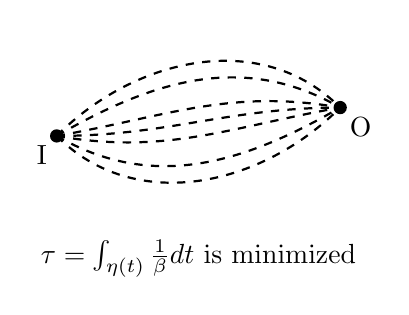
\begin{tikzpicture}[scale=1.2]
    % Define points S and O
    \coordinate (I) at (0,0);
    \coordinate (O) at (3,0.3);
    
    % Draw points S and O
    \fill (I) circle (2pt) node[below left] {I};
    \fill (O) circle (2pt) node[below right] {O};
    
    % Draw multiple paths between S and O
    % Upper paths
    \draw[dashed,thick] (I) to[out=10,in=170] (O);
    \draw[dashed,thick] (I) to[out=30,in=150] (O);
    \draw[dashed,thick] (I) to[out=45,in=135] (O);
    
    % Middle paths
    \draw[dashed,thick] (I) to[out=0,in=180] (O);
    
    % Lower paths
    \draw[dashed,thick] (I) to[out=-10,in=-170] (O);
    \draw[dashed,thick] (I) to[out=-30,in=-150] (O);
    \draw[dashed,thick] (I) to[out=-45,in=-135] (O);
    
    % Add figure label
    \node at (1.5,-1.3) {$\tau = \int_{\eta(t)} \frac{1}{\beta} dt$ is minimized};
\end{tikzpicture}
\end{center}

\noindent This principle was generalized to the Lagrangian Principle, which states that for a mechanical system, described by position $(q^{1}, \dots, q^{n})$ and velocity $(\dot{q}^{1}, \dots, \dot{q}^{n})$, we can construct a scalar function $\mathcal{L}(q^{i}, \dot{q}^{i})$ called the Lagrangian, such that its integral, called the action, is stationary for $\eta(t)$ in the space of possible paths. 

\begin{equation}
\delta S = \delta \left[ \int_{\eta(t)} \mathcal{L} dt \right] = 0
\tag{The Variational Principle}
\label{VariationalCondition}
\end{equation}
\noindent One may show this condition is equivalent to $\mathcal{L}$ satisfying the following differential equation: 

\begin{align}
\frac{\partial \mathcal{L}}{\partial q^{i}} - \frac{d}{dt} \frac{\partial \mathcal{L}}{\partial \dot{q}^{i}} = 0 \text{ for all coordinates } q^{i} 
\tag{The Euler-Lagrange Equations}
\end{align}

\noindent Now, suppose we are given a scalar quantity, $H$ called the Hamilitonian, such that:
\begin{equation}
    \dot{p}_i = -\frac{\partial H}{\partial q^i} 
    \quad \mbox{and} \quad 
    \dot{q}^i = \frac{\partial H}{\partial p_i}
\end{equation}

\noindent Consider the expression:
\begin{equation}
\mathcal{L} = \sum_{i} p_{i} \dot{q}^{i} - H
\label{eq:Hamiliton}
\end{equation}

\noindent Applying the definitions, it follows that:

\begin{align}
\frac{\partial \mathcal{L}}{\partial q_{i}} = -\frac{\partial H}{\partial q_{i}} \text{ and } \frac{\partial \mathcal{L}}{\partial \dot{q}_{i}} = p_{i} \text{ imply } && \frac{\partial \mathcal{L}}{\partial q^{i}} - \frac{d}{dt} \frac{\partial \mathcal{L}}{\partial \dot{q}^{i}} = 0
\tag{A New Formula for $\mathcal{L}$}
\end{align}

\noindent Therefore, \ref{eq:Hamiliton} is the Lagrangian for a mechanical system. The action $S$ for this mechanical system is then written: $S = \int_{t} p_{i} dq^{i} - H dt \label{SymplecticPot}$. 
Symplectic geometry was invented to study the term $\theta = p_{i} dq^{i}$ in the integral of $S$. Namely, the symplectic form, the primary tool of symplectic geometry, is defined to be $\omega = -d \theta$. 

\begin{remark}
From the integral based intuition for $\omega$ - understanding $\omega$ is equivalent to understanding how the integral $S$ behaves
\end{remark}

\noindent \textbf{References: } \textcite{Arnold2010}, \textcite{Terek2020}, \textcite{Feynman:1494701}

\subsection{Delzant's Correspondence Theorem}
In this thesis, we describe how a scalar function generates vector fields One structure that we impose is a Lie group action on our manifold. Now, when a Lie group $G$ acts on a manifold $M$, it establishes an orbit map $\sigma_{p}: G \to M$. This map can be differentiated at the identity of $G$, giving rise to a linear transformation $\left( d \sigma_{p} \right)_{e} \colon \mathfrak{g} \to T_p M$, where $\mathfrak{g}$ is the Lie algebra of $G$. Define the action field corresponding to $X \in \mathfrak{g}$ to be $X^{\#}_{p} = \left( d \sigma_{p} \right)_{e} X$. For each vector field, we ask the question: Does there exist a function which generates this vector field? These functions are known as moment maps and are crucial to the symplectic framework. 

\begin{figure}[htbp]
    \centering
    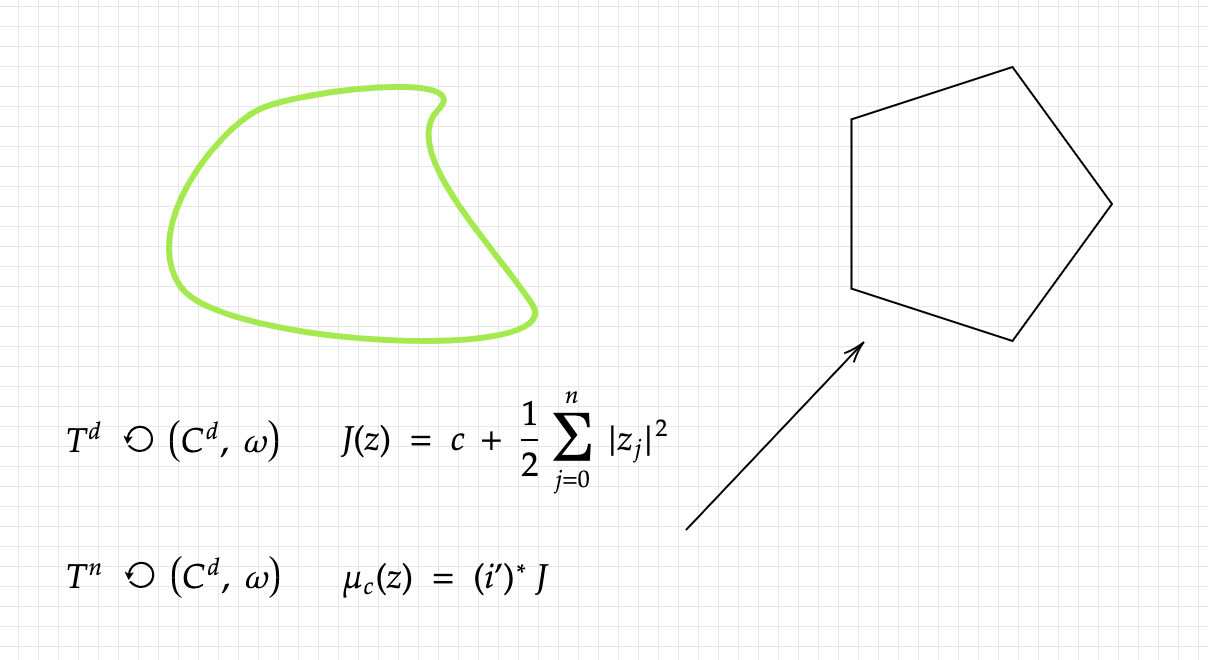
\includegraphics[width=.6\linewidth]{Chapters/Figures/Screenshot 2025-02-05 at 8.59.25 PM.png}
    \caption{Identifying polytopes $\Delta$ as images of moment maps via Delzant's Theorem.}
    \label{fig:delzant_theorem}
\end{figure}

\noindent One classical result in symplectic geometry is Delzant's Correspondence Theorem. It states that there is a one-to-one correspondence between symplectic toric manifolds and Delzant polytopes --- the latter arise as images of moment maps associated with the former. Denote a polytope $\Delta$. Then its corresponding Delzant space is $(X_{\Delta}, \omega)$. Delzant's Theorem is quite interesting because it establishes that the images of momentum maps themselves are geometric objects. Understanding what happens for more general Hamiltonian $G$-spaces (where $G$ is any compact and connected Lie group, not necessarily the torus) is one of the most challenging problems in symplectic geometry. 

\begin{figure}[htbp]
    \centering
    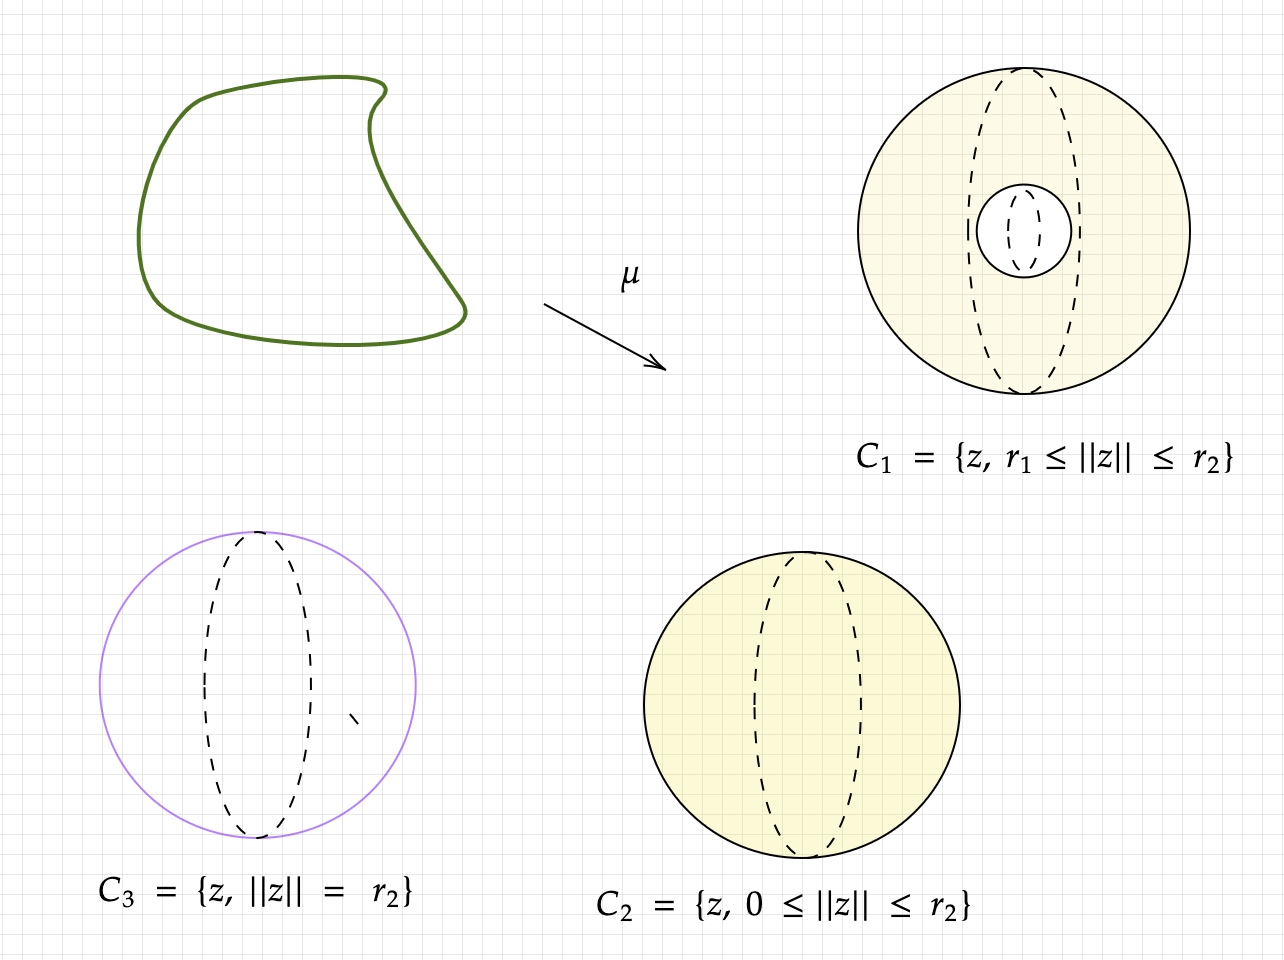
\includegraphics[width=.6\linewidth]{Chapters/Figures/Screenshot 2025-02-06 at 9.44.33 AM.png}
    \caption{Possibilities of nontrivial moment-images when $\text{SO}(3) \circlearrowright M$.}
    \label{fig:so3_moment_images}
\end{figure}

\noindent Now, our investigation starts with the simplest compact and connected non-Abelian group: the special orthogonal group $\text{SO}(3)$. The moment-images for (compact and connected) Hamiltonian $\text{SO}(3)$-spaces, which are necessarily $\text{SO}(3)$-invariant subsets of $\mathfrak{so}(3)^*\cong \mathbb{R}^3$, can then only fall into one among four cases: the origin, a sphere, a closed ball, or a closed hollow ball. It is easy to construct examples showing that all four possibilities do occur, but to which precise extent does this image determine the original space? What is a Delzant correspondence for Hamiltonian $\text{SO}(3)$-spaces, if there is even one at all? \bigskip 

\noindent \textbf{References: } \textcite{AtiyahGS1982}, \textcite{Delzant1988}, \textcite{Blaom1996}



\chapter{Background}


\theoremstyle{plain} %italicizes text
\newtheorem{theorem}{Theorem}[section]
\newtheorem{prop}[theorem]{Proposition}
\newtheorem{lemma}[theorem]{Lemma}
\newtheorem{cor}[theorem]{Corollary}
\newtheorem{conj}[theorem]{Conjecture}
\newtheorem*{claim}{Claim}
\newtheorem*{question}{Question}
\newtheorem*{conv}{Convention}

\theoremstyle{remark}
\newtheorem{exr}{Exercise}
\newtheorem*{rmk}{Remark}

\theoremstyle{defn}

\newtheorem*{FTA}{Fundamental Theorem of Algebra}


\section{Symplectic Manifolds and Hamiltonian Actions}

In this section, we will see the prototypical examples for symplectic manifolds, and discuss with more precision the definitions that guide the subject. This section will answer the questions:

\begin{enumerate}
    \item How does one define classical Mechanics?
    \item What is a symplectic manifold and what are its technicalities?
    \item How does one define rigorously a Lie group action?
    \item How to define Hamiltonian actions?
\end{enumerate}

\subsection{Classical Mechanics}
Classical mechanics studies rigid bodies. Symplectic geometry is modeled after classical mechanics. Therefore, we define several notions in classical mechanics. Each classical mechanical system has an underlying geometry $Q$. This is where motion takes place:

\begin{defn}[Configuration Space of a Mechanical System]
The configuration space of a mechanical system is a smooth manifold $Q$, called the configuration manifold. 
\end{defn}

\noindent Furthermore, for motion to occur, we require both position and momentum to be well defined:

\begin{defn}[Positions and Momenta]
Given a configuration space $Q$, the position $q = (q^{1}, \dots, q^{n})$ 
of a mechanical element is a coordinate pair made up of smoothly valued chart functions on $Q$. Given a chart $(U, q)$ on $Q$, we have that $q: U \to \mathbb{R}^{k}$, where $k = \dim U$. Momenta of the mechanical system on the other hand are are linear maps on the cotangent space: $(T_{x} Q)^{*}$. Identifying basis vectors of the cotangent space $(T_{x} Q)^{*}$ in charts as $\frac{\partial}{\partial q^{i}}$, we have that: $p = \sum_{i} p_{i} \frac{\partial}{\partial q^{i}}$ and $p: T_{x} U \to \mathbb{R}^{k}$. 
\end{defn}

\noindent One key distinction in symplectic geometry versus classical Newtonian mechanics is that in symplectic geometry, when we work on a configuration space $Q$, position coordinates are valued in $Q$, while momentum vectors to $x \in Q$ are valued in $(T_{x} Q)^{*}$, the dual space to $T_{x} Q$. The reason for this distinction comes from Riemannian geometry. When our manifold $Q$ has a Riemannian metric $g$, we will show that momentum is valued in $(T_{x} Q)^{*}$, where $x \in Q$. 

\begin{defn}[Kinetic Energy using $g$]
Given a Riemannian manifold $(Q, g)$, kinetic energy $E$ is an inner product valued on its tangent space $T_{x} Q$. The inner product is:

$$E = T_{x} Q \times T_{x} Q \to \mathbb{R}, \; E = \frac{m}{2} \langle \cdot, \cdot \rangle$$
\end{defn}

\begin{remark}
Let $q, \dot{q}$ be the position and velocity of a particle. This definition of kinetic energy generalises the formula $E = \frac{m}{2} |\dot{q}|^2$ to configuration space $Q$. In classical mechanics, it is also common to write $E = \frac{1}{2} pv$. We require a new definition of momentum, $p$.  
\end{remark}

\begin{defn}[Momentum as a Linear Map]
Define momentum to be: $p = \langle \dot{q}, \cdot \rangle$. Therefore, $p \in T_{x} Q^{*}$, and $E = \frac{1}{2} p(\dot{q})$ 
\end{defn}

\begin{remark}
When $(Q,g)$ is a Riemannian manifold, it is clear that for $x \in Q$, momentum is $p \in (T_{x} Q)^{*}$. This definition also allows us to define momentum even if the configuration space $Q$ does not possess a Riemannian metric. 
\end{remark}

\begin{defn}[Phase Space of a Mechanical System]
The phase space of a mechanical system is the manifold which contains all of the information necessary to describe mechanical motion. The phase space of classical mechanical system is $T^{*} Q$:

$$T^{*} Q = \bigsqcup_{q \in Q} T^{*}_{q} Q = \{(q, d \phi) \in T_{q} Q^{*} \}$$ 
\end{defn}

\begin{lemma}
\label{CotangentBundle}
The phase space of a classical mechanical system is a vector bundle $\pi: T^{*} Q \to Q$, where $\pi (q, d \phi) = q$
\end{lemma}

\begin{proof}
For a chart $(x, U)$ on $Q$, we must define a bundle chart, $h_{x}: \pi^{-1}(U) \to U \times \mathbb{R}^{n}$. The following choice of bundle chart suffices:

$$h_{x}: \pi^{-1}(U) \to U \times (\mathbb{R}^{n})^{*} \cong U \times (\mathbb{R}^{n}): (q, d \phi) \to (q, D(\phi x^{-1}) \circ x(q))$$ 
using the definition of $d \phi$ in coordinates. For the next isomorphism, we use the canonical isomorphism between $\mathbb{R}^{n}$ and $(\mathbb{R}^{n})^{*}$. In addition, it must be shown that the map $h_{x}$ also induces an isomorphism between fibres $\pi^{-1}(q) \cong \mathbb{R}^{n}$. This occurs as the map $D(\phi x^{-1}) \circ x(q)$ has full rank. Therefore, for each $p \in Q$, there is an open set $U$, a homeomorphism $h: \pi^{-1} U \to U \times \mathbb{R}^{n}$ such that
\[
\begin{tikzcd}
& U \times \mathbb{R}^{n} \arrow[d, "\pi"] \\
\pi^{-1}(U) \arrow[ru, "h"] \arrow[r, "\pi|_{\pi^{-1}(U)}"] & U
\end{tikzcd}
\]
\noindent Such that the diagram commutes, and the composite map: $h_{q}: \pi^{-1}(q) \to \{q\} \times \mathbb{R}^{n} \to \mathbb{R}^{n}$ is a vector space isomorphism. 
\end{proof}

\begin{defn}[Definition of a Mechanical System]
A mechanical system $(Q, H)$ is a configuration space $Q$, a phase space $T^{*} Q$, and a smooth scalar function on the phase space $H: T^{*} Q \to \mathbb{R}$. Time evolution of the mechanical system is governed by the \textit{Hamilton Equations}:

$$\dot{q} = \frac{\partial H}{\partial p}, \; \dot{p} = -\frac{\partial H}{\partial q}$$

\noindent Alternatively, we can write them in each coordinate as: $\dot{q}^{i} = \frac{\partial H}{\partial p_{i}}, \; \dot{p}_{i} = -\frac{\partial H}{\partial q^{i}}$.

\end{defn}

\begin{lemma}[Model Space for Symplectic Geometry]
\label{VecDefn}
Consider the mechanical system $(Q, H)$, and its phase space $T^{*} Q$. Consider the vector field: 

\begin{equation}
X_{H} = \frac{\partial H}{\partial p_{i}} \frac{\partial}{\partial q^{i}} - \frac{\partial H}{\partial q^{i}} \frac{\partial}{\partial p_{i}}
\end{equation}
\noindent Define the symplectic form $\omega$, on $T^{*} Q$ to be:
$$\omega = \sum_{i \geq 1} dq^{i} \wedge dp_{i}$$
\noindent Then we have the following: $\omega(X_{H}, \cdot) = dH$.
\end{lemma}

\begin{proof}
Writing out the evaluation: 
$$\omega(X_{H}, \cdot) = \sum_{i \geq 1} \left( \frac{\partial H}{\partial p_{i}} \frac{\partial}{\partial q^{i}} - \frac{\partial H}{\partial q^{i}} \frac{\partial}{\partial p_{i}} \right) \left[ dq^{i} \wedge dp_{i} \right] = \frac{\partial H}{\partial p_{k}} dp_{k} + \frac{\partial H}{\partial q^{k}} dq^{k} = dH $$

\noindent The last step follows from the chain rule, appLied to $H: T^{*} Q \to \mathbb{R}$.
\end{proof}

\begin{remark}
This reformulation of Hamilton's equations also works in the reverse direction. 
\end{remark}

Now, we would like to show the opposite direction. To do so, we want to be able to invert $\omega(X_{H}, \cdot) = dH$. Therefore, we make the following definition:

\begin{defn}
A symplectic form $\omega$ is non-degenerate if when vector field $Z$ satisfies $\omega(Z, X) = 0$ for all $X \in \mathfrak{X}(T^{*} Q)$, then $Z = 0$ everywhere. Namely, if $\omega$ is non-degenerate, then for any $x \in Q$

\begin{align}
\omega_{x}^{-1}: (T_{x} Q)^{*} \to T_{x} Q \text{ given by } \left [ \omega(v, \cdot) \to v \right] \text{ is an isomorphism}.
\end{align}
\end{defn}

\begin{remark}
When a symplectic form is non-degenerate, this has the unique consequence that its inverse, $\omega^{-1}$ is well-defined and therefore unique. 
\end{remark}

\begin{lemma}[Non-degeneracy of $\omega$]
Given a configuration space $Q$, for its phase space $T^{*} Q$, the symplectic form:
$$\omega = \sum_{i \geq 1} dq^{i} \wedge dp_{i}$$
is non-degenerate. 
\end{lemma}

\begin{proof}
Suppose a vector field $Z$ satisfies $\omega(Z, X) = 0$ for all $X \in \mathfrak{X}(T^{*} Q)$. Let $Z = \alpha(q, p) \frac{\partial}{\partial q^{i}} + \beta \frac{\partial}{\partial p_{i}}$. Then, we choose $X^{1} = \frac{\partial}{\partial q^{i}}$ and $X^{1} = \frac{\partial}{\partial p_{i}}$. We note that: 

\begin{align}
\omega(Z, X^{1}) = \alpha(q,p) = 0 && \omega(Z, X^{2}) = \beta(q,p) = 0  
\end{align}

\noindent Therefore, $Z = 0$ and $\omega$ is non-degenerate
\end{proof}

\begin{defn}[Integral Curve on $T^{*} Q$]
Consider the configuration manifold $Q$, and its phase space $T^{*} Q$. 
Given a vector field $X_{H} \in \mathfrak{X}(T^{*} Q)$, the integral curve of that vector field is $\gamma(t) = (\gamma_{1}, \dots, \gamma_{n})$, such that: $\dot{\gamma_{j}} = X_{H}(\gamma)_{j}$.
\end{defn}

\begin{lemma}[Reverse Implication]
Consider the mechanical system $(Q, H)$, and its phase space $T^{*} Q$. Let  $\omega$ be defined as above, such that: $\omega(X_{H}, \cdot) = dH$. Then the integral curve of $X_{H}$, $\gamma(t)$ satisfies Hamilton's equations. 
\end{lemma}
Let: $\gamma(t) = (q^{1}(t), \dots, q^{n}(t), p_{1}(t), \dots, p_{n}(t))$
be the integral curve of $X_{H}$. Since $\omega$ is non-degenerate, its inverse is unique. So, we have that $X_{H}$ has the same definition as in \ref{VecDefn}.

\begin{proof}
\noindent Now, according to the definition of an integral curve: $\dot{\gamma_{j}} = \left[ X_{H}(\gamma) \right]_{j}$

\noindent Matching coefficients, we have:
\begin{align}
\dot{\gamma}_{i} \frac{\partial}{\partial q^{i}} = \frac{\partial H}{\partial p_{i}} \frac{\partial}{\partial q^{i}} && \dot{\gamma}_{i+n} \frac{\partial}{\partial p_{i}} = -\frac{\partial H}{\partial q^{i}} \frac{\partial}{\partial p_{i}}
\end{align}

\noindent Unraveling the definition $\dot{\gamma}_{i} = \frac{dq^{i}}{dt}$ and $\dot{\gamma}_{i+n} = \frac{dp_{i}}{dt}$, we have that: 

\begin{align}
\dot{q}^{i} = \frac{\partial H}{\partial p_{i}} && \dot{p_{i}}  = -\frac{\partial H}{\partial q^{i}} 
\end{align}

\noindent Therefore, the equations of motion of a classical mechanical system $(Q, H)$ and the equation $\omega(X_{H}, \cdot) = dH$ on $T^{*} Q$ are equivalent.
\end{proof}

\begin{remark}
\label{OverviewOfSymp}
A generalization of classical mechanics would to be study a manifold $M$, with a closed, non-degenerate two form $\omega$, a smooth function $H: M \to \mathbb{R}$, and vector fields $X_{H}$ such that $\omega(X_{H}, \cdot) = dH$. This would mimic a classical system and replicate it in the case that $M = T^{*} Q$, and $\omega = \sum_{i \geq 1} dq^{i} \wedge dp_{i}$. This generalization of classical mechanics is symplectic geometry and will be developed in the following section. 
\end{remark}

\noindent \textbf{References}: \textcite{Bjorn2018}, \textcite{Terek2020}, \textcite{Arnold2010}

\subsection{Symplectic Structures}
As in \ref{OverviewOfSymp}, symplectic geometry studies manifolds equipped with a two form $(M, \omega)$ which have the model geometry of $T^{*} Q$. As usual in differential geometry, for this construction we must describe objects on the linear level before moving to the global level.  

\begin{defn}[Symplectic Vector Space]
A symplectic vector space $V$ is a pairing $(V,\Omega)$, where $V$ is a vector space, and $\Omega: V \times V \to \mathbb{R}$ is a non-degenerate skew-symmetric bilinear form. Here, non-degeneracy means that $\Omega(v, w) = 0$ for all $w \in V$ if and only if $v = 0$.
\end{defn}

\begin{remark}
The symplectic prototype resembles $T^{*} Q$, as that geometry came equipped with another skew-symmetric, bilinear form, namely $\omega$.
\end{remark}

\begin{remark}[A Bilinear Form is just a Skew-Symmetric Matrix]
A non-degenerate skew-symmetric bilinear form is just a skew-symmetric matrix, when we fix a choice of basis. Therefore, we can take the prototypical symplectic manifold to have the off-diagonal skew-symmetric identity matrix. 
\end{remark}

\begin{example}[Symplectic Vector Space Prototype of $\mathbb{R}^{2n}$]
\label{SymVectorPrototype}
The prototypical symplectic vector space is the vector space $(\mathbb{R}^{2n}, \Omega = \begin{bmatrix}
    0 & \operatorname{Id}_{n} \\
    -\operatorname{Id}_{n} & 0
\end{bmatrix})$ with the standard bases. One computes $\Omega(v,w)$ according to the following prescription: $\omega(v,w) = v^{T} \Omega w \in \mathbb{R}$.
\end{example}

\begin{lemma}[Vector Space Prototype is Well-defined]
The symplectic vector space prototype is non-degenerate, bilinear and skew-symmetric.
\end{lemma}

\begin{proof}
The expression $\left[ (v,w) \to v^{T} \Omega w \right]$ is bilinear, by matrix composition of the row space, versus the column space. Now, to show the symplectic prototype $\Omega$ is skew-symmetric. Consider the standard basis for $\mathbb{R}^{2n}$, that is $\mathcal{B} = \{ (1, 0, \dots, 0), (0, 1, \dots, 0), \dots (0, 0, \dots, 1) \}$ written as: 
$$\mathcal{B} = \{ e_{1}, \dots e_{n}, h_{1}, \dots, h_{n} \} $$
We note that on bases, $\Omega$ is:
\begin{align}
\Omega(e_{j}, h_{j}) = 1 && \Omega(h_{j}, e_{j}) = -1 && \Omega(h_{i}, h_{j}) = \Omega(e_{i}, e_{j}) = 0
\end{align}

\noindent Therefore, $\Omega$ is skew-symmetric on bases. By bilinearity, it is skew symmetric on $V \times V$. Additionally, as $\Omega$ has determinant $1$, it establishes an isomorphism $\Omega^{-1}: V^{*} \to V$, and we note that as a result, $\Omega$ is non-degenerate.
\end{proof}

\begin{remark}
To build a symplectic manifold, the generalization of classical mechanics based on the model geometry $T^{*} Q$, we want each of the tangent spaces to a manifold $M$, to be isomorphic the symplectic prototype, and the symplectic form on our manifold $M$, $\omega$ to be the prototype symplectic form in each tangent space as well.
\end{remark}

\begin{remark}
In \ref{SymplecticPot}, we took an approach to the symplectic form in a different way, where we defined it as negative the exterior derivative of the symplectic potential $\theta$. From this intuition, we require another condition on $\omega$, which is that it is closed. This is because the exterior derivative operator satisfies $d^2 = 0$. In general, whenever a two form is closed, we can always write it as an exterior derivative of a one form locally, so the symplectic potential will always make sense. To understand this further see: \textcite{Terek2020}. 
\end{remark}

\begin{defn}[Definition of a Symplectic Manifold]
A symplectic manifold $(M, \omega)$ is a smooth manifold $M$, equipped with a two form $\omega \in \Omega^2(M)$, that is closed, non-degenerate, and skew-symmetric. 
\end{defn}

\begin{example}[Sympletic Geometry of $(\mathbb{C}^{n}, \omega)$]
\label{ComplexForm}
Let $z = (z_{1}, \dots, z_{n})$, where each $z_{j} = x_{j} + i y_{j}$. 
Making note of the isomorphism $\mathbb{C}^{n} \cong \mathbb{R}^{2n}$, there exists the non-degenerate, skew-symmetric, bilinear form inherited from $\mathbb{R}^{2n}$ \ref{SymVectorPrototype}. Then: $\omega_{\mathbb{R}^{2n}} = dx_{1} \wedge dy_{1} + \dots + dx_{2} \wedge dy_{n}$. It is an observation that:

$$d \overline{z}_{j} \wedge dz_{j} = \left[ dx_{j} - i dy_{j} \right] \cdot \left[ dx_{j} + i dy_{j} \right] = i dx_{j} \wedge dy_{j}$$

\noindent Therefore, we define $\omega_{\mathbb{C}^{n}} = \frac{-i}{2} \sum_{j \geq 1} \overline{dz}_{j} \wedge dz_{j}$. 
\end{example}

\begin{example}[Sympletic Geometry of a Surface in $\mathbb{R}^{3}$]
\label{SurfaceForm}
Let $M \subset \mathbb{R}^3$ be a orientable surface, $M$ is an embedded manifold in $\mathbb{R}^{3}$. Since $M$ is an orientable surface, it admits a normal vector field $x \to N_{x}$. Therefore, a skew-symmetric form on $M$ is the area form of $M$: $\omega_{x}(v,w) = \langle N_{x}, v \times w \rangle$. 
\end{example}

\begin{lemma}[Surface Form]
The area form on a surface $\omega$ \ref{SurfaceForm} is a skew-symmetric, non-degenerate, bilinear form
\end{lemma}

\begin{proof}
Let's prove $\omega$ is non-degenerate. Let $v, w \in \mathfrak{X}(M)$. Let $v_{x}, w_{x}$ be the tangent vectors at $x \in M$. Suppose $\omega(v, w) = 0$ for all $w \in \mathfrak{X}(M)$. Then:

$$\langle N_{x}, v_{x} \times w_{x} \rangle = 0$$

\noindent Since $\langle \; \cdot, \cdot \; \rangle$ is non-degenerate, and $N_{x} \neq 0$, we have for all $w_{x} \in T_{x} M$

$$v_{x} \times w_{x} = 0$$

\noindent Choose $w_{x}$ perpendicular to $v_{x}$ in the plane of $T_{x} M$. Then, $v_{x} = 0$. Therefore, $v = 0 \in \mathfrak{X}(M)$. It follows from an observation that $\omega$ is skew-symmetric. We observe that:

$$\omega(v,w) = -\omega(w,v)$$

\noindent Finally, since the cross product is bilinear, we conclude. 
\end{proof}

\noindent \textbf{References}: \textcite{Terek2020}, \textcite{Bjorn2018}

\subsection{No Local Invariants of Symplectic Manifolds}

It is important to see how diffeomorphisms alter the symplectic form. As usual in differential geometry, we study the case when diffeomorphisms preserve the symplectic form:

\begin{defn}[Pullback of a symplectic form]
Suppose we are given a symplectic manifolds $(M', \omega')$ and $(M', \omega')$, vectors $v, w \in T_{x} M$, and a point $x \to \phi(x) = x'$. If we have a diffeomorphism $\phi: M \to M'$, the pullback of $\omega'$, denoted $\phi^{*} \omega'$ is the map:

$$\phi^{*} \omega_{x'}'(v,w) = \omega_{x'}'(d \phi_{x} v, d \phi_{x} w)$$
\end{defn}

\begin{defn}[Symplectomorphism]
Given two symplectic manifolds $(M, \omega)$ and $(M', \omega')$, a symplectomorphism $\phi$ between them is a diffeomorphism $\phi$ such that for any point $x \in M$, $v, w \in T_{x} M$:
$$\left[ \phi^{*} \omega_{x'}' \right](v,w) = \omega_{x}(v,w)$$

\begin{center}
\begin{tikzcd}[row sep=large, column sep=large]
    M \arrow[r, "\phi"] \arrow[d, "x \to \; \omega_{x}"'] & M' \arrow[d, "x' \to \; \omega_{x'}'"] \\
    \Lambda^2(T^*M) & \Lambda^2(T^*M') \arrow[l, "\phi^*"]
\end{tikzcd}

\end{center}

\noindent A symplectomorphism is a map $\phi$ which makes the following diagram commute.
\end{defn}

\noindent In each of the above examples \ref{SurfaceForm} and \ref{ComplexForm}, the symplectic forms all were (up to relabeling):
\[ \omega = \sum_{j \geq 1} dq^{j} \wedge dp_{j} \]

\begin{remark}[No Local Invariants]
Was this by accident? One observation early on in symplectic geometry was that all symplectic manifolds are in fact locally symplectomorphic, we will see this in the following theorem \ref{Darboux}.
\end{remark}

\begin{theorem}[Darboux's Theorem -- All Symplectic Manifolds are Locally Symplectomorphic]
\label{Darboux}
Let \((M, \omega)\) be a symplectic manifold, and \(p \in M\) be any point. Then, there is a chart \((U, (x^1, \dots, x^n, y^1, \dots, y^n))\) around \(p\) for which: $\omega = \sum_{j \geq 1} dx_{j} \wedge dy_{j}$
All symplectic manifolds locally look the same, and there are no local invariants in symplectic geometry. 
\end{theorem}

For a proof of \ref{Darboux}, see \cite{Arnold2010}. This is an important result, since it allows us to take the canonical local coordinates when we need to do so.  

\subsection{Algebras of Vector Fields}

We defined a symplectic manifold $(M, \omega)$ based on the model geometry of the bundle: $T^{*} Q \to Q$. On the manifold $T^{*} Q$, we reformulated classical mechanics in terms of the symplectic form there \ref{VecDefn}.

\begin{remark}
This reformulation of classical mechanics can also be done for a symplectic manifold $(M, \omega)$. 
\end{remark}

The generalization of Hamilton's equations becomes the definition of a Hamilitonian vector field.

\begin{defn}[Hamiltonian Vector Field]
\label{HamilitonianVectorField}
Let $(M, \omega)$ be a symplectic manifold, then, a vector field $X_{H} \in \mathfrak{X}(M)$ is called Hamiltonian if there exists a smooth Hamilitonian function $H: M \to \mathbb{R}$ such that $\omega(X_{H}, \cdot) = dH$.
\end{defn}

\noindent Since $\omega$ is non-degenerate, $\omega^{-1}$ exists and 
$X_{H} = \omega^{-1} dH$. A weaker notion than a Hamilitonian vector field is a symplectic vector field. Such a vector field does not necessarily derive from a Hamilitonian function $H$. 

\begin{defn}[Symplectic Vector Field]
Let $(M, \omega)$ be a symplectic manifold, then, a vector field $X \in \mathfrak{X}(M)$ is called symplectic if $\omega(X, \cdot)$ is closed. 
\end{defn}

\begin{lemma}[Inclusion Law]
Every Hamilitonian vector field is a symplectic vector field.
\end{lemma}

\begin{proof}
Note that $\omega(X_{H}, \cdot) = dH$, which is closed. 
\end{proof}

\begin{remark}
Symplectic vector fields and Hamilitonian vector fields form algebras with composition laws. To see these, we first define function composition on our symplectic manifold. Function composition occurs via the Poisson-bracket $\{\cdot, \cdot \}$
\end{remark}  

\begin{defn}[Poisson Bracket]
\label{PoissonBracket}
Consider a symplectic manifold $(M, \omega)$. Let $f, g$ be two smooth functions $f, g: M \to \mathbb{R}$, and $X_{f}$ and $X_{g}$ be the corresponding Hamilitonian vector fields. The Poisson bracket between $f$ and $g$ is a map: 
\begin{align}
\{\cdot, \cdot\}: C^{\infty}(M) \times C^{\infty}(M) \to C^{\infty}(M) && \{f, g \} = \omega(X_{f}, X_{g})
\end{align}

\end{defn}

\begin{lemma}[Lie Bracket is the Poisson Bracket]

Given Hamilitonian vector fields $X_{f}$ and $X_{g}$, as defined in \ref{PoissonBracket}, we have that:

$$[X_{f}, X_{g}] = X_{f} X_{g} - X_{g} X_{f} = -X_{\{f, g \}}$$ 
\end{lemma}

\begin{proof}
Lemma is proved in appendix: \ref{PoissonIsLie}
\end{proof}

\begin{defn}[Algebras of Vector Fields]
Consider a symplectic manifold $(M, \omega)$. Let $\mathcal{S}(M, \omega, [\cdot, \cdot])$ and $\mathcal{H}(M, \omega, [\cdot, \cdot])$ denote the algebras of Symplectic and Hamilitonian vector fields on $M$
\end{defn}

\begin{lemma}[Sym Algebra is Well-Defined]

Let $(M, \omega)$ be a symplectic manifold as above. We first show that $\mathcal{S}(M, \omega, [\cdot, \cdot])$ is closed under the Lie-bracket $[\cdot, \cdot]$. 
\end{lemma}

\begin{proof}
Note that if $X, Y \in \mathfrak{X}(M)$ is symplectic, $\omega(X, \cdot)$ is closed. For some $x \in M$, consider a small neighborhood $V$, where $x \in V$. Since $X$ is symplectic, we write: $\omega(X, \cdot) = df'$, where $df': V \to \mathbb{R}$ is a smooth function. We do the same for $Y$, writing $\omega(X, \cdot) = dg'$. Therefore, we understand that $X$ and $Y$ are locally Hamilitonian, and so we write: $[X, Y] = -X_{\{f', g' \}}$. It suffices to note that $\{f', g' \}$ now is the symplectic function for $[X, Y]$. 
\end{proof}

\begin{lemma}[Ham Algebra is Well-Defined]

Let $(M, \omega)$ be a symplectic manifold as above. We show that $\mathcal{H}(M, \omega, [\cdot, \cdot])$ is closed under the Lie-bracket $[\cdot, \cdot]$. 
\end{lemma}

\begin{proof}
This proof follows from the above argument for $\mathcal{S}(M, \omega, [\cdot, \cdot])$, noting that now when $f, g$ are functions $M \to \mathbb{R}$, $\{f, g \}$ is also a function $M \to \mathbb{R}$
\end{proof}

\noindent \textbf{References:} \textcite{Terek2020}, \textcite{Bjorn2018}, \textcite{Arnold2010}

\subsection{Lie Group Actions}
One natural question in manifold theory is whether a Hamilitonian $H$ can generate a symmetry from its dynamics. 

\begin{remark}
These are made explicit by having a Lie group $G$, act on the manifold. The Lie group action, establishes a method of studying the action of symmetry.
\end{remark}

\begin{defn}[Lie Group Action]
Let $G$ be a Lie group, and $M$ be a manifold. A smooth, left action of $G$ on $M$, denoted $G \circlearrowright M$ is a smooth map: $G \times M \to M$ given by $(g,x) \mapsto g \cdot x$ satisfying $e \cdot x = x$ and $g \cdot (h \cdot x) = (gh) \cdot x$.
\end{defn}

\begin{example}[Toric Action $T^{n} \circlearrowright \mathbb{C}^{n}$]
One common Lie group action is that of the torus, $T^{n}$ acting on $\mathbb{C}^{n}$: 
\begin{equation}
(e^{i \beta_{1}}, \dots, e^{i \beta_{n}}) \cdot (e^{i \theta_{1}}, \dots, e^{i \theta_{n}}) = (e^{i (\theta_{1} + \beta_{1})}, \dots, e^{i (\theta_{n} + \beta_{n})})
\end{equation}
The toric action is given by phase rotation in each of the complex coordinates. 
\end{example}

\noindent To each Lie group element $G$, there exists an associated mapping:

\begin{defn}[Orbit Map]
Consider a symplectic manifold $(M, \omega)$ with a Lie-group action $G \circlearrowright M$. Given any point $x \in M$, we define the orbit map $\sigma_{x}: G \to M$ to be the map $[g \to g \cdot x]$. 
\end{defn}

\begin{defn}[Classifying Lie Group Actions]
\noindent Let $G \circlearrowright M$ be a Lie group action on a manifold:
\begin{enumerate}
    \item Given $x \in M$, $G \cdot x = \{g \cdot x: g \in G \}$ is the \textit{orbit} of $x$.
    \item Given $x \in M$, $G_{x} = \{g \in G: g \cdot x = x\}$ is the \textit{stabilizer} of $x$.
    \item The action is \textit{transitive} if there is an $x \in M$ such that $G \cdot x = M$.
    \item The action is \textit{free} if $G_{x} = e$ for all $x \in M$.
    \item The action is \textit{proper} if the enriched action $G \times M \to M \times M$ is a proper map.
    \item The action is \textit{effective} if $g \cdot x = x$ for all $x \in M$ impLies that $g = e_{G}$.
\end{enumerate}
\end{defn}

\noindent Since a Lie-group action $G \circlearrowright M$ is smooth, the orbit map is differentiable. 

\begin{defn}[Lie Algebra of $G$, $\mathfrak{g}$]
The Lie Algebra of $G$, $(\mathfrak{g}, [ \cdot, \cdot])$ is the tangent space to $G$ at the identity, $e$: $\mathfrak{g} = T_{e} G$. The composition rule in $\mathfrak{g}$ is given by $[ \cdot, \cdot]$, which is the Lie bracket on $\mathfrak{g}$.
\end{defn}

\noindent Consider the conjugation map: $\Psi_{g}: G \to G$ given by:  

$$\Psi_{g}(h) = gh g^{-1}$$

\noindent Since the action of $G \circlearrowright G$ is smooth, we take its derivative at the identity:

$$\left(d \Phi_{g}(X)\right)_{e}: T_{e} G \to T_{e} G$$

\noindent Then, the map: $g \to \left(d \Phi_{g}(X)\right)_{e}$ can be differentiated at the identity.

\begin{align}
\operatorname{ad}_{X}(Y): T_{e} G \times T_{e} G \to \mathbb{R} && \operatorname{ad}_{X}(Y) = \left[X, Y \right]    
\end{align}

\begin{defn}{Lie bracket on $G$, $[ \cdot, \cdot ]$}
The Lie-bracket is the quantity: 

$$\operatorname{ad}_{X}(Y) = \left[X, Y \right]$$
\end{defn}

\noindent The Lie bracket will be important in the study of the Lie algebra of $\mathfrak{so}(3)$. Since $G \circlearrowright M$ is smooth, the derivative of the orbit map at the identity is well defined:

\begin{defn}[Derivative of the Orbit Map]
Given a symplectic manifold $(M, \omega)$, and a Lie group action $G \circlearrowright M$, and a point $x \in M$, the orbit map $\sigma_{x}$ can be differentiated at the identity to yield the map:

$$\left( d \sigma_{x} \right)_{e}: \mathfrak{g} \to T_{x} M$$
\end{defn}

\begin{defn}[Fundamental Vector Field]
Let $X \in T_{e} G$. The vector field $X^{\#}$ is the image of $X$, as $x$ ranges over $M$:

$$X^{\#} = \bigsqcup_{x \in M} \left( d \sigma_{x} \right)_{e}(X) $$
\end{defn}

\begin{example}[Action of $S^{1} \circlearrowright S^{1}$, What is $X^{\#}_{\theta_{1}}$]

Consider a symplectic manifold $(S^{1}, \omega)$, acted on by a Lie-group action 

\begin{align}
S^{1} \circlearrowright S^{1} \text{ via } [e^{i \theta} \cdot e^{i \theta_{1}} \to e^{i(\theta + \theta_{1})} ]
\end{align}

\noindent In this case, $\sigma_{x}(\theta) = e^{i \theta} x$, and $(d \sigma_{x})_{e} = ix$. Since $ix = X^{\#}_{\theta_{1}}(x)$, we deduce that $X^{\#}_{\theta_{1}} = \frac{\partial}{\partial \theta_{1}}$.
\end{example}

\begin{center}
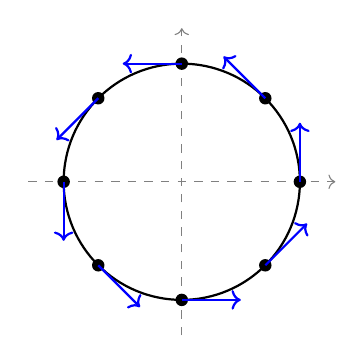
\begin{tikzpicture}[scale=1.5]
    % Draw the circle S^1
    \draw[thick] (0,0) circle (1);
    
    % Add coordinate axes for reference
    \draw[gray,dashed,->] (-1.3,0) -- (1.3,0);
    \draw[gray,dashed,->] (0,-1.3) -- (0,1.3);
    
    % Draw tangent vectors at fewer points
    \foreach \angle in {0, 45, 90, 135, 180, 225, 270, 315} {
        % Calculate position on circle
        \coordinate (P\angle) at (\angle:1);
        
        % Draw point
        \fill (P\angle) circle (1.5pt);
        
        % Draw longer tangent vector (rotated 90 degrees from radius)
        % The vector field X^#_θ = i·e^{iθ} points perpendicular to the radius
        \draw[->,thick,blue] (P\angle) -- +({90+\angle}:0.5);
    }
\end{tikzpicture}

\end{center}

\begin{remark}
We want to study which Hamiltonian-type functions generate a $X^{\#}$ field. These questions we will begin to answer in the next section. 
\end{remark}

\subsection{Hamiltonian Actions}

\begin{defn}[Comoment Map $\mu_{c}$]

Consider a symplectic manifold $(M, \omega)$, and a Lie group action $G \circlearrowright M$. Denote the Lie algebra of $G$ as $\mathfrak{g}$. Then, the comoment map generates fundamental vector fields $X^{\#}$ on $\mathfrak{X}(M)$. 

\begin{align}
\mu_{c}: \mathfrak{g} \to C^{\infty}(M) && X_{\mu_{c}(X)} = X^{\#}
\end{align}

\noindent An equivalent condition is that $d \mu_{c}(X) = \omega(X^{\#}, \cdot)$.
\end{defn}

\begin{remark}
The co-moment map $\mu_{c}$ contains the information about every Hamilitonian function generating fundamental vector fields on $M$. 
\end{remark}

\begin{defn}[Moment Map $\mu$]
There is a natural dual to $\mu: M \to \mathfrak{g}$
\end{defn}

\begin{lemma}[Moment-Comoment Duality]
\noindent The comoment and moment maps are connected via the relation:

$$\left[\mu_{c}(X) \right](p) = \mu^{X}(p)$$
\end{lemma}

\begin{defn}[Symplectic Action]
Let $(M, \omega)$ be a symplectic manifold, with a smooth Lie group action $G \circlearrowright M$. A smooth action $G \circlearrowright M$ is a symplectic action if for each $g \in G$, the map $g: M \to M$ is a symplectomorphism. We denote a symplectic action $(M, \omega, G)$
\end{defn}

\begin{defn}
 A symplectic action $G \circlearrowright (M, \omega)$ is called a Hamiltonian action if there exists a linear $\mu_{c}: \mathfrak{g} \to C^{\infty}(M)$, the comoment map, such that the diagram commutes:
\begin{center}
\begin{tikzcd}
(\mathfrak{g}, [\cdot, \cdot]) \arrow[r, "\mu_c"] \arrow[d, "\#"] &
(C^\infty(M), \{\cdot, \cdot\}_\omega) \arrow[d, "X_{\cdot}"] \\
(\mathcal{S}(M, \omega), [\cdot, \cdot]) & \arrow[l, hook]
(\mathcal{H}(M, \omega), [\cdot, \cdot])
\end{tikzcd}
\end{center}
\end{defn}
\noindent Therefore, a symplectic action is Hamiltonian if its corresponding vector field is itself Hamiltonian, such that the diagram commutes. 
\begin{example}[Symplectic Action but not Hamilitonian]
An action that is not Hamiltonian is rotation on the torus, $S^{1} \circlearrowright T^{2}$:
\begin{equation}
S^{1} \circlearrowright T^{2}: \theta \circ (\theta_{1}, \theta_{2}) = (\theta_{1} + \theta, \theta_{2})
\end{equation}
\end{example}
The vector field induced by this action is $\frac{\partial}{\partial \theta_{1}}$. Taking $\omega = d\theta_{1} \wedge d\theta_{2}$, we have that $\omega(\frac{\partial}{\partial \theta_{1}}, \cdot) = d\theta_{2}$. Note $i_{\frac{\partial}{\partial \theta_{1}}} \omega = d\theta_{2}$ cannot be everywhere written as the exterior derivative of a Hamiltonian function. Otherwise, we would have for all $z \in S^{1}$, that $d\theta_{2}$ is exact, violating the cohomological restriction $H^{1}_{dR}(S^{1}) = \mathbb{R}$. 
\begin{example}[Rotation on $S^{2}$]
An action that is Hamiltonian is rotation on the sphere $S^2$, around the $\hat{z}$ axis.
Let $S^{2} \subset \mathbb{C} \times \mathbb{R}$, where $S^{2} = \{(z, h): |z|^2 + h^2 = 1 \}$. Define the action of $S^{1} \circlearrowright S^{2}$ by: 
\begin{equation}
S^{1} \circlearrowright S^{2}: \theta \circ (z, h) = (e^{i \theta} z, h) 
\end{equation}
The symplectic form for this action is $d\theta \wedge dh$, where this is the area form in polar coordinates. The vector field is $\frac{\partial}{\partial \theta}$. Therefore, we may declare that $\mu_{c} = h$, and $d\mu_{c} = \omega(X_{\theta}, \cdot)$.
\end{example}


\begin{example}[Generalization of Angular Momentum]
The Lie group action $S^1 \circlearrowright \mathbb{C}$ generates the black arrows as a vector field. The action is explicitly: 
\begin{equation}
S^1 \circlearrowright \mathbb{C}: e^{i\beta} \cdot re^{i\theta} \mapsto re^{i(\theta + \beta)}
\end{equation}
As in differential geometry, vectors are the directional derivatives they induce. Therefore, in polar coordinates the black arrows are the vector field such that:
\begin{equation}
X(e^{i\theta}) = i \cdot e^{i\theta}
\end{equation}
Therefore, $X^{\#}(\theta, r) = \frac{\partial}{\partial \theta}$. The symplectic form on $\mathbb{R}^2$ is the canonical area form in polar coordinates, $\omega = r d\theta \wedge dr$. Now, $d\mu_{c} = r dr$. We find that $\mu_{c} = \frac{r^2}{2}$. Considering a particle moving along the path with mass $1/2$, we note that in fact our expression $\mu_{c}$ is the classical angular momentum of the particle.
\begin{equation}
|\mu_{c}| = L_{\theta}
\end{equation}

\end{example}

\noindent \textbf{References:} \textcite{Terek2020}, \textcite{Bjorn2018}, \textcite{Arnold2010}, \textcite{Silva2001}

\subsection{Properties of Hamiltonian G-Spaces}

An important operation when establishing moment map images is the following:

\begin{defn}[Minkowski Sum]
Given two vector spaces $A, B$, their Minkowski sum is $A + B = \{a + b: a \in A, b \in B \}$, where $+$ is the vector space addition operator.
\end{defn}

\begin{remark}
A key lemma we will use throughout this thesis is the following: for the product of two manifolds, the moment image of the sum of spaces will be the Minkowski sum of the individual moment images. This is proven below:
\end{remark} 

\begin{lemma}[Moment of Product is Minkowski Sum]
Let \((M_1, \omega_1, G, \mu_1)\) and \((M_2, \omega_2, G, \mu_2)\) be two Hamiltonian \(G\)-spaces. It holds that 
\((M_1 \times M_2, \omega_1 \oplus \omega_2, G, \mu_1 \oplus \mu_2)\) is also a Hamiltonian \(G\)-space, where the action of $G$ on \(M_1 \times M_2\) is diagonal and the action of the new moment map $\mu_1 \oplus \mu_2: M_1 \times M_2 \rightarrow \mathfrak{g}^*$ is given by $(\mu_1 \oplus \mu_2)(x, y) \doteq \mu_1(x) + \mu_2(y)$. In particular, $(\mu_1 \oplus \mu_2)(M_1 \times M_2) = \mu_1(M_1) + \mu_2(M_2)$, an observation that we will apply later \end{lemma}
Let $i_{x_{2}}(x) = (x, x_{2})$, and $i_{x_{1}}(x) = (x_{1}, x)$ be the inclusion maps. Using the fact that $T(M_{1} \times M_{2}) = \pi_{1}^{*}TM_{1} \oplus \pi_{2}^{*}TM_{2}$, we have that if $f \in C^{\infty}(M_{1} \times M_{2})$ then:
\begin{equation}
X_f|_{(x_1, x_2)} = X_{f \circ i_{x_2}}^{\omega_1} + X_{f \circ i_{x_1}}^{\omega_2}
\end{equation}
\begin{equation}
d(\mu_1 \oplus \mu_2)_{(x_{1}, x_{2})}(\cdot) = (\pi_{1}^{*}\omega_{1} \oplus \pi_{2}^{*}\omega_{2})(X_{f(i_{x_{2}})}^{\omega_{1}} + X_{f(i_{x_{1}})}^{\omega_{2}}, \cdot)
\end{equation}
Since opposite projections cancel, i.e., $d\pi_{1}d\pi_{2} = 0$, we have that the moment map is diagonal, and:
\begin{equation}
(\mu_1 \oplus \mu_2)_{(x_{1}, x_{2})} = \mu_{1}(x_{1}) + \mu_{2}(x_{2})
\end{equation}

\begin{example}[Moment Image of $S^{2}(r_{2}) \times S^{2}(r_{1})$]

Consider $(S^{2}(r_{2}), \mu_{2})$ where $\mu_{2}(r) = r$, and $(S^{2}(r_{1}), \mu_{1})$ given by $\mu_{2}(r) = r$. This is proven here \ref{MomentMapIsInclusion}. Then, $(\mu_1 \oplus \mu_2)_{(x_{1}, x_{2})} = \mu_{1}(x_{1}) + \mu_{2}(x_{2})$. 

\begin{align}
(\mu_1 \oplus \mu_2)(S^{2}(r_{2}) \times S^{2}(r_{1})) = B(r_{2} + r_{1}) \setminus B(|r_{2} - r_{1}|) 
\end{align}

\end{example}

\noindent \textbf{References:} \textcite{Arnold2010}, \textcite{Silva2001}, \textcite{Terek2020}

\chapter{Delzant's Theorem}
\section{Delzant's Theorem}

In this section we cover the following:
\begin{enumerate}
    \item What is the statement and proof of Delzant's Theorem
    \item Delzant in the $[-1, 1] = \Delta$ case
    \item Delzant's Theorem and uniqueness modulo toric equivariant symplectomorphism
\end{enumerate}
\subsection{Toric Actions and Moment Maps}

Toric actions are the most elementary Lie group actions because they are abelian. Let's see the definition of a toric action on complex $\mathbb{C}^{d}$-space:   
\begin{example}[Toric Action $T^{n} \circlearrowright \mathbb{C}^{n}$]
\label{ToricAction}
One common Lie group action is that of the torus, $T^{n}$ acting on $\mathbb{C}^{n}$: 
\begin{equation}
(e^{i \beta_{1}}, \dots, e^{i \beta_{n}}) \cdot (e^{i \theta_{1}}, \dots, e^{i \theta_{n}}) = (e^{i (\theta_{1} + \beta_{1})}, \dots, e^{i (\theta_{n} + \beta_{n})})
\end{equation}
The toric action is given by phase rotation in each of the complex coordinates. 
\end{example}

\noindent A toric action will also have a corresponding vector field. This is important to study as it will be used to find the moment map $\mu_{c}$

\begin{lemma}[Fundamental Vector Field $X^{\#}$ of Toric Action] 
Given a toric action as in \ref{ToricAction}, $$X^{\#}_{\theta_{1}, \dots \theta_{n}} = \frac{\partial}{\partial \theta_1} + \dots + \frac{\partial}{\partial \theta_n}$$
\end{lemma}

\begin{proof}
We take the derivative and observe:

\begin{align}
\left[ d \sigma_{\theta_{1}, \dots, \theta_{n}} \right]_{e} = (i e^{i \theta_{1}}, \dots, i e^{i \theta_{n}})
\end{align}

\noindent But this is the vector field tangent to $e^{i \theta_{1}}, e^{i \theta_{2}}, \dots e^{i \theta_{n}}$. This is, in local coordinates:

$$X^{\#}_{\theta_{1}, \dots \theta_{n}} = \frac{\partial}{\partial \theta_1} + \dots + \frac{\partial}{\partial \theta_n}$$
\end{proof}

Now, we must compute the symplectic form in polar coordinates. This is:

\begin{lemma}[A Symplectic Form on $\mathbb{C}^{n}$]
We choose a symplectic form:
$$\omega = \sum_{i} dz_{i} \wedge d\overline{z_{i}} = \sum_{i} |z_i| d \theta_{i} \wedge d|z_{i}|$$
\end{lemma}

\begin{proof}
In \ref{ComplexForm}, we proved that: $\omega_{\mathbb{C}^{k}} = \frac{-i}{2} \sum_{k} dz \wedge \overline{dz}$ was a symplectic form for $(\mathbb{C}^{k}, \omega_{\mathbb{C}^{k}})$. We choose a multiple of this form to be our form:

$$\omega = \sum_{j \geq 1} dz_{j} \wedge d\overline{z_{j}} $$

\noindent Then, we use polar coordinates $dz_{j} = |z_{j}| d \theta_{j}$, and find

$$\omega = \sum_{j \geq 1} |z_j| d \theta_{i} \wedge d|z_{j}|$$
\end{proof}

Now, with a symplectic form $\omega$, and a fundamental vector field, we compute the moment map $\mu_{c}$ on $\mathbb{C}^{d}$. This is:

\begin{lemma}[Moment Map for $(\mathbb{C}^{d}, \omega, T^{d})$]
\label{ComplexMomentMap}
\begin{equation}
\left (\mu (z_{1}, \dots, z_{n}) \right)_{j} = \frac{|z_{j}|^2}{2} + \lambda_{j}
\end{equation}

\noindent Where $\lambda_{j} \in \mathbb{R}^{*}$
\end{lemma}

\begin{proof}
According to $d \mu_{c} = \omega(X^{\#}, \cdot)$, we observe that: 
$\left (d \mu_{c} \right)_{j} = \left[ \omega(X^{\#}_{\theta_{1}, \dots \theta_{n}}, \cdot) \right]_{j} = |z_{j}| \cdot d|z_{j}|$. We integrate both sides to find: $\left (\mu \right )_{j} = \frac{|z_{j}|^2}{2} + \lambda_{j} \in (\mathbb{R}^{d})^{*}$
\end{proof}

\noindent \textbf{References:} \textcite{Guillemin1994} \textcite{Terek2020}, \textcite{Silva2001}

\subsection{Definitions Concerning the Delzant Construction}

\begin{remark}
Now, with basic results behind us for the toric action $T^{d} \circlearrowright M$, we can study the geometry of the image of the moment map as in \textcite{Delzant1988}. 
\end{remark}

Delzant's construction is an association between a symplectic manifold with toric action: $(M_{\Delta}, \omega_{\Delta}, T^{d})$ to each Delzant space $\Delta$, where $\Delta$ is a type of polytope, called a Delzant polytope. Delzant's construction links $M_{\Delta} \leftrightarrow \Delta$ via the Delzant moment map. Now, we will study the construction:

\begin{remark}
In this case, we denote the Delzant construction moment map: $J: M_{\Delta} \to (\mathbb{R}^{d})^{*}$, where as the moment map $\mu_{c}$ denotes the one here $\ref{ComplexMomentMap}$.
\end{remark}

\begin{defn}[Delzant Polytope]
A Delzant polytope $(\Delta, n, d)$ is a convex polytope in $(\mathbb{R}^{n})^{*}$. There are $d$-faces of a Delzant polytope $\Delta$, and $n$ edges meeting in each vertex $p$. The edges meeting at each $p$ are rational. Furthermore, $v_{1}, \dots, v_{n}$ can be chosen to be a basis of $(\mathbb{Z}^{n})^{*}$. Each one of these faces is defined by a normal equation, where $u_{i}$ is the inward pointing normal vector to each face \textcite{Delzant1988}

\begin{equation}
\langle u_{i}, x \rangle \geq \lambda_{i}, \; i \in \{1, \dots, d \}
\end{equation}
\end{defn}

\noindent Now, we define several maps used in the Delzant construction:

\begin{lemma}[Delzant Quotient Map]
Let $e_{1}, \dots, e_{d}$ be standard basis vectors of $\mathbb{R}^{d}$. There exists a linear map $\pi'$: 

$$\pi': T^{d} \to T^{n}$$
\end{lemma}

\begin{proof}
Let $e_{1}, \dots, e_{d}$ be standard basis vectors of $\mathbb{R}^{d}$ and consider the map:
\begin{equation}
\pi: \mathbb{Z}^{d} \to \mathbb{Z}^{n} 
\end{equation}
Consider its natural extension by inclusion:
\begin{equation}
\pi: \mathbb{R}^{d} \to \mathbb{R}^{n} 
\end{equation}
Then, there exists a quotient map: $\pi': T^{d} \to T^{n}$, such that the diagram commutes. The quotient map: $\pi'$ does the following:
\begin{equation}
\pi': [r] \mapsto [\pi(r)] 
\end{equation}
\begin{center}
\begin{tikzcd}
    \mathbb{Z}^{d} \arrow[r, "\pi"] \arrow[d, hook] & \mathbb{Z}^{n} \arrow[d, hook] \\
    \mathbb{R}^{d} \arrow[r, "\pi"] \arrow[d, two heads] & \mathbb{R}^{n} \arrow[d, two heads] \\
    T^{d} \arrow[r, "\pi'"] & T^{n}
\end{tikzcd}
\end{center}
\end{proof}

\begin{remark}
\label{NSpaceRemark}
It is an instructive exercise that $\pi'$ has a less obvious form. Let the coordinates of each normal vector be $u_{i} = (u_{i,1}, \dots, u_{i,n})$. Then,
\begin{equation}
\pi'(z_{1}, \dots, z_{d}) \mapsto (\prod_{i=1}^{d} z_{i}^{u_{i,1}}, \dots, \prod_{i=1}^{d} z_{i}^{u_{i,n}})
\end{equation}
\end{remark}

Since $\pi'$ is a linear map, we study its kernel, which we define here:

\begin{defn}[Delzant $N$ Space]
Let the kernel of $\pi'$ be $N$. 
\end{defn}

\begin{lemma}[Exact Sequence Defining $N$]
$\mathfrak{n}$ can equivalently be defined by the exact sequence:

$$0 \to \mathfrak{n} \to \mathbb{R}^{d} \to \mathbb{R}^{n} \to 0  $$
\end{lemma}
\begin{proof}
This follows from the exact sequence:
$$0 \to N \to T^{d} \to T^{n} \to 0$$
\noindent Now we take the differential of each map and move to the Lie algebra level:

$$0 \to \mathfrak{n} \to \mathbb{R}^{d} \to \mathbb{R}^{n} \to 0  $$
\noindent The conclusion follows
\end{proof}

\noindent \textbf{References}: \textcite{Silva2001} \textcite{Guillemin1994}, \textcite{Terek2020}

\subsection{Construction of Delzant Space $M_{\Delta}$ given $\Delta$}

Now, for a polytope $\Delta \in (\mathbb{R}^{n})^{*}$, we will construct a symplectic manifold $M_{\Delta}$, such that its moment map $J: M_{\Delta} \to \Delta$. First we need a few definitions:

\begin{defn}[Delzant Inclusion Map]
$$i: N \to T^{d}$$
\end{defn}

\begin{defn}[Dual Inclusion Map]
Define: 
\begin{align}
i^{*}: (\mathbb{R}^{d})^* \to \mathfrak{n}^{*} \text{ where } i^{*} \text{ is the derivative transpose of } i
\end{align}
\end{defn}

\begin{lemma}[Almost $M_{\Delta}$] 
The set $(i^{*} \circ J)^{-1}(0)$ is a compact subset of $\mathbb{C}^{d}$, \\
and $N$ acts freely on this set.
\end{lemma}

\begin{proof}
From the exact sequence:
\begin{equation}
0 \to \mathfrak{n} \to \mathbb{R}^{d} \to \mathbb{R}^{n} \to 0  
\end{equation}
we conclude that $\ker i^{*} = \operatorname{Im} \pi^{*}$. Furthermore, it is an observation that:  
\begin{equation}
\label{ImageofMDelta}
(i^{*} \circ \mu_{c})^{-1}(0) = \mu_{c}^{-1}(\pi^{*}(\Delta))
\end{equation}
Note that the stabilizer group of $z$ in $T^{d}$ is $T^{I}$, where $I$ is the number of $0$'s in the coordinate expansion of $z$. Note when $p$ is in the interior of $\Delta$, the number of $0$'s for a given $z_{i}$ is zero. This is because:
\begin{equation}
p \in \operatorname{Int} \Delta \Longleftrightarrow \langle u_{i}, p \rangle > \lambda_{i}
\end{equation}
When $p$ a vertex of the polygon, assume $p=0$, so that:
\begin{equation}
\langle u_{i}, p \rangle = 0, \; i \in \{1, \dots, n \}
\end{equation}
Then, we note that $\pi(T^{I}) \cong T^{n}$ and therefore, we have that $T^{I} \cap N = \emptyset$. Since $T^{I}$ is also the stabilizer group, we have that $N$ acts freely at $z$. Furthermore, note that since $J$ is proper, $(i^{*} \circ J)^{-1}(0)$ is compact.  
\end{proof}

\begin{remark}
In order to define the Delzant Space $M_{\Delta}$, we need to remove the free action of $N$ on $(i^{*} \circ \mu_{c})^{-1}(0)$. For this, we cite the following Theorem. 
\end{remark}

\begin{theorem}[Marsden-Weinstein] 
\label{Marsden-Weinstein}
Let $(M, \omega, G, \mu)$ be a Hamiltonian $G$-space and $p \in \mathfrak{g}^*$ be a regular value for $\mu$. Assume that the action $G_p \circlearrowright \mu^{-1}(p)$ is free and proper. Then the quotient $\mu^{-1}(p)/G_p$ has a unique symplectic form $\omega_0$ characterized by the relation $\pi^*\omega_0 = i^*\omega$, where $\pi: \mu^{-1}(p) \rightarrow \mu^{-1}/G_p$ is the quotient projection and $i: \mu^{-1}(p) \hookrightarrow M$ is the inclusion. We call $(\mu^{-1}(p)/G_p, \omega_0)$ the reduction of $(M, \omega)$ to level $p$. For more details, see \textcite{MarsdenWeinstein1974} and \textcite{Terek2020}
\end{theorem}

The following lemma is important as we reduce:

\begin{lemma}[Moment Map of Lie Subalgebra]
\label{MomentMapLieSubAlgebra}
Let $\mathfrak{g}$ be a Lie algebra and $\mathfrak{h} \subseteq \mathfrak{g}$ a Lie subalgebra. Suppose a symplectic manifold $(M, \omega)$ is equipped with a Hamiltonian action of a Lie group $G$ with moment map 
\[
\mu_c: M \to \mathfrak{g}^*.
\]
Let $H \subseteq G$ be a Lie subgroup with Lie algebra $\mathfrak{h}$, and consider the restricted action $H \circlearrowright M$. Then the dual of the inclusion map $i: \mathfrak{h} \hookrightarrow \mathfrak{g}$ induces a projection
\[
i^*: \mathfrak{g}^* \to \mathfrak{h}^*,
\]
and the composition
\[
\mu_H := i^* \circ \mu: M \to \mathfrak{h}^*
\]
is a moment map for the $H$-action.
\end{lemma}

\begin{proof}
Since Hamiltonian functions arising from the restricted action $H \circlearrowright M$ are restrictions of Hamiltonian functions arising from $G \circlearrowright M$, it follows that:
\begin{align}
\mu_{H, c}: \mathfrak{h} \to C^{\infty}(M) &&  \mu_{c}: \mathfrak{g} \to C^{\infty}(M) 
\end{align}
\noindent are related by $\mu_{H, c} = \mu_{c} \circ i$. Then, we note that: $\langle \mu, i \circ X \rangle = \mu_{H,c}(X)$. Therefore, $\langle i^{*} \circ \mu, X \rangle = \mu_{H,c}(X)$, and we note that: $\mu_{H} = i^{*} \circ \mu$. 
\end{proof}

\begin{theorem}[Construction of $M_{\Delta}$]
Given $\Delta \in( \mathbb{R}^{n})^{*}$ a Delzant Polytope, there exists: 
$(M_{\Delta}, \omega_{0}, T^{n})$ such that $J(M_{\Delta}) = \Delta$
\end{theorem}

\begin{proof}
From the Marsden-Weinstein Theorem \ref{Marsden-Weinstein}, 
we reduce $\mathbb{C}^{d}$ with respect to $N$. Since $N$ acts freely on $(i^{*} \circ J)^{-1}(0)$, the reduced space is a smooth symplectic manifold, which we declare $M_{\Delta}$. The symplectic manifold $M_{\Delta}$ admits a $T^{n}$ action after reduction. Define $\mu_{c}$ to be the moment map $\mu_{c}$ arising from the action of $T^{n}$ on $M_{\Delta}$. Consider the inclusion $i': \mathbb{R}^{n} \to \mathbb{R}^{d}$ and its transpose, $(i')^{*}: (\mathbb{R}^{d})^{*} \to (\mathbb{R}^{n})^{*}$. By \ref{MomentMapLieSubAlgebra}, the moment image of $M_{\Delta}$ is by $\ref{ImageofMDelta}$, $J(M_{\Delta}) = \Delta$
\begin{align}
J = (i')^{*} \circ \mu_{c} && M_{\Delta} = (i^{*} \circ \mu_{c})^{-1}(0)/N && J(M_{\Delta}) &\cong \Delta \in \mathbb{R}^{n}^{*}
\end{align} 
\end{proof}

\noindent \textbf{References}: \textcite{Silva2001} \textcite{Guillemin1994}, \textcite{Terek2020}

\subsection{Delzant Construction for $\Delta = [-1,1]$}

We will do the Delzant Construction for $\Delta = [-1,1]$. 

\begin{question}[What is $N$ given $\Delta$]
Claim: $N = \{(t, t) : t \in [0, 2\pi)\}$.
\end{question}
\begin{proof}
When $\Delta = [-1,1]$, the normal vectors are $u_{1} = -1$ and $u_{2} = 1$. In this case, $N = \ker \pi'$ where:
\begin{equation}
\pi'(z_{1}, z_{2}) = z_{1}^{-1} z_{2}
\end{equation}
\noindent We use Remark \ref{NSpaceRemark}, and observe that $N = \{(t, t) : t \in [0, 2\pi)\}$.
\end{proof}
\begin{question}[What is $\mu$ given $\Delta$]
Claim: $J(z) = \frac{(|z_{1}|^2, |z_{2}|^2)}{2} + (-1, -1) $
\end{question}
\begin{proof}
Since the interval $\Delta$ can also be seen as $x \geq -1$ and $-x \geq -1$ we have that $\lambda_{1} = -1$ and $\lambda_{2} = -1$.
Using \ref{ComplexForm}, the complex space $\mathbb{C}^{2}$ has moment map: $\mu(z) = \frac{(|z_{1}|^2, |z_{2}|^2)}{2} + (-1, -1)  $
\end{proof}
\begin{question}[What is $J$ given $\Delta$]
Claim: $J = i^{*} \circ J = \frac{|z_{1}|^2 + |z_{2}|^2}{2} - 2$
\end{question}
\begin{proof}
Note that $i: \mathfrak{n} \to \mathbb{R}^2$, given by $v \mapsto (v,v)$. Note that $\langle i^{*}(z_{1}, z_{2}), v \rangle = \langle (z_{1}, z_{2}), (v, v) \rangle = (z_{1} + z_{2}) v$. We use the property that $\langle a^{*} w, v \rangle = \langle w, av \rangle$.
Therefore, $i^{*}(z_{1}, z_{2}) = z_{1} + z_{2}$, and we note that:
$$i^{*} \circ J = \frac{|z_{1}|^2 + |z_{2}|^2}{2} - 2$$
\end{proof}
\begin{question}[What is $M_{\Delta}$]
Claim: $M_{\Delta} \cong \mathbb{C} P^{1}$
\end{question}
\begin{proof}
We note that $N \cong U(1)$. Therefore, $X_{\Delta} \cong S^{3}/N \cong S^{3}/U(1) \cong \mathbb{CP}^{1}$. 
\end{proof}

\subsection{Convexity of Moment Maps}
For the other direction, we use the \textcite{AtiyahGS1982}. Following the treatment in \textcite{Silva2001}, we sketch only one part of the proof. 
\begin{theorem}[Atiyah-Guillemin-Sternberg] 
Let \((M, \omega)\) be a compact connected symplectic manifold, and let \(T^{m}\) be an \(m\)-torus. Suppose that \(\psi: T^{m} \to \operatorname{Symp}(M, \omega)\) is a Hamiltonian action with moment map \(\mu: M \to \mathbb{R}^{m}\). Then:
\begin{enumerate}
    \item the levels of \(\mu\) are connected;
    \item the image of \(\mu\) is convex;
    \item the image of \(\mu\) is the convex hull of the images of the fixed points of the action.
\end{enumerate}
\end{theorem}
Consider the statements:
\begin{enumerate}
    \item $A_{n}$ - the levels of $\mu$ are connected for any $T^{n}$ action
    \item $B_{n}$ - the image of $\mu$ is convex for any $T^{n}$ action
\end{enumerate} From Morse Theory, we have that $A_{1}$ and $B_{1}$ hold.

\begin{theorem}[Part of Proof of AGS]
$A_{m-1}$ implies $B_{m}$
\end{theorem}

\begin{proof}
\noindent Consider a moment map $\mu$ from a toric action $T^{n} \circlearrowright M$. We can consider the toric action of an $(n-1)$-dimensional sub-torus on $M$, $T^{n-1} \circlearrowright M$, by using an injective matrix $A \in \mathbb{Z}^{n \times (n-1)}$ and defining:
\begin{align}
\psi_{A}: T^{n-1} &\to \operatorname{Symp}(M, \omega) && \theta \mapsto \psi_{A\theta}
\end{align}

\noindent Since $A^{T}: \mathbb{R}^{n} \to \mathbb{R}^{n-1}$ is a linear map from the Lie algebra of the torus onto the Lie algebra of its subgroup, the moment map of $\psi_{A}$ is $\mu_{A} = A^{T} \mu$. Consider $p, p_{0} \in \mu_{A}^{-1}(\xi)$, then $A^{T} \mu(p) = \xi = A^{T} \mu(p_{0})$. Now it follows that:

\begin{equation}
\mu_{A}^{-1}(\xi) = \{p \in M: \mu(p) - \mu(p_{0}) \in \operatorname{Ker}(A^{T}) \}
\end{equation}
\noindent Since $\mu_{A}^{-1}(\xi)$ is a connected manifold for regular value $\xi$ and is locally path connected, the inverse image is path connected. Therefore, for a path $t \mapsto p_{t} \in \mu_{A}^{-1}(\xi)$, there also exists a path $t \mapsto \mu(p_{t}) - \mu(p_{0}) \in \operatorname{Ker}(A^{T})$. Since $\operatorname{Ker}(A^{T})$ is $1$-dimensional, it follows that all elements $\mu(p_{t})$ must be a linear superposition of $\mu(p_{0})$ and $\mu(p_{1})$ - two points determine a line!

\begin{equation}
(1-t) \mu(p_{0}) + t \mu(p_{1}) \in \mu(M), \; t \in [0,1]
\end{equation}
Choosing points $p_{0}$ and $p_{1}$ closely approximated by rational $p_{0}'$ and $p_{1}'$ we run this argument again - finding a matrix which contains $\mu(p_{0}') - \mu(p_{1}')$ in its kernel. Taking limits, we find that $\mu(M)$ is convex.
\end{proof}

\noindent \textbf{References}: \textcite{Silva2001}, \textcite{Delzant1988}, \textcite{Terek2020}

\subsection{Uniqueness of Delzant Spaces}
Now, we have shown that for each Delzant polytope, there exists a corresponding Delzant space, and given a Delzant space, we may find the polytope. Actually, the association of $\Delta$ and $M_{\Delta}$ is unique, up to toric-equivariant symplectomorphism as in  \textcite{Delzant1988}.

\begin{defn}
Given a Delzant polytope $\Delta$, if there exist moment maps $\mu_1$ and $\mu_2$, and Delzant spaces, $X_{\Delta, 1}$ and $X_{\Delta, 2}$, such that there exists an isomorphism $\gamma: \operatorname{Im}(\mu_1) \to \operatorname{Im}(\mu_2)$ and $\phi: X_{\Delta, 1} \to X_{\Delta, 2}$ is a $\gamma$-equivariant symplectomorphism, then $\phi$ is called a $\gamma$-equivariant symplectomorphism, which is a diffeomorphism in the symplectic category that respects the moment maps.
\end{defn}
\begin{center}
\begin{tikzcd}
X_{\Delta, 1} \arrow[r, "\phi"] \arrow[d, "\mu_1"'] & X_{\Delta, 2} \arrow[d, "\mu_2"] \\
\operatorname{Im}(\mu_1) \arrow[r, "\gamma"'] & \operatorname{Im}(\mu_2)
\end{tikzcd}
\end{center}

\noindent Now, we would like to extend these results to the non-Abelian case $G \circlearrowright M$. It turns out that so long as the action of $G$ has regular values, the uniqueness of the moment map image is determined by the toric (Abelian) part of $G$, which is known as the maximal torus of $G$. 

\noindent \textbf{References: } \textcite{Blaom1996}, \textcite{GuilleminSternberg1982}.

\newpage

\setcounter{section}{4}

\chapter{Moment Maps for $\rm{SO}(3)$-actions}
\section{Moment Maps of Lie Actions Arising from $\mathrm{SO}(3)$}
Now, we would like to begin developing a generalization of Delzant's  Theorem for a symplectic manifolds admitting a Hamilitonian $\mathrm{SO}(3)$ action, $(M, \omega, \rm{SO}(3))$. 

\begin{remark}
As a result, the moment map for such an action will be $\mu: M \to \mathfrak{so}(3)^{*}$. As a result, we must study the Lie algebra $\mathfrak{so}(3)^{*}$
\end{remark}

\noindent In this section we cover the following: 

\begin{enumerate}
    \item Coadjoint action $\rm{SO}(3)$ is given by evalulation
    \item The Lie-algebra isomorphism $ \mathfrak{so}^{*}(3) \cong \mathbb{R}^{3}$
    \item The classification of moment images of symplectic manifold with Hamilitonian $\mathrm{SO}(3)$ action, $(M, \omega, \rm{SO}(3))$. 
\end{enumerate}

\subsection{Coadjoint Action}

To classify moment map images, we must first show that the natural action of $\rm{SO}(3)$ on $\mathfrak{so}(3)$ is itself given by evaluation. 

\begin{defn}[Coadjoint Action]
Given a Lie group $G$, and its Lie algebra $\mathfrak{g}$, there is a natural action of $G \circlearrowright \mathfrak{g}$ given by the coadjoint action. For each covector $h \in \mathfrak{g}^{*}$, $A \cdot h \to \operatorname{Ad}_{A^{-1}}^{*} h$
\end{defn}

\begin{lemma}\label{lem:so3-isomorphism}
The map $\Phi: \mathfrak{so}(3)^{*} \to \mathbb{R}^{3}$ defined by
\[
\Phi(\xi) = \left( \xi(E_{1}), \xi(E_{2}), \xi(E_{3}) \right)
\]
\noindent is an $\mathrm{SO}(3)$-equivariant vector space isomorphism.
\end{lemma}

\begin{proof}
Since $\dim \mathfrak{so}(3) = \dim \mathfrak{so}(3)^* = 3$, it suffices to show that $\Phi$ is injective. Suppose $\Phi(\xi) = 0$. Then $\xi$ vanishes on the basis $\{E_1, E_2, E_3\}$ of $\mathfrak{so}(3)$, so $\xi = 0$. Hence, $\ker \Phi = 0$, and $\Phi$ is injective.
\end{proof}

\begin{remark}
Now, we would like to prove that the coadjoint action on $\mathfrak{so}(3)^{*}$ is given by evaluation. 
\end{remark}

\begin{lemma}[Coadjoint Action is Given by Evaluation]
\label{ActionEvalulation}
Let $\xi \in \mathfrak{so}(3)^{*}$, and $\Phi$ the evaluation map as above. Then:
\[
\Phi\left( \xi \circ \mathrm{Ad}_{A^{-1}} \right) = A \Phi(\xi)
\]
\end{lemma}

\begin{proof}
Under the isomorphism $\Phi$, and noting that $A^{-1} = A^{T}$ for $A \in \mathrm{SO}(3)$, we want to show \label{AdInvariance} $A \Phi(\xi) = \left( \xi(A^{T} E_{1} A),\; \xi(A^{T} E_{2} A),\; \xi(A^{T} E_{3} A) \right)$. Let $\xi(E_1) = \xi_1$, $\xi(E_2) = \xi_2$, and $\xi(E_3) = \xi_3$. It suffices to verify \eqref{AdInvariance} on the basis elements. We verify this for the first basis element, the other cases follow by a similar computation. 

\begin{align}
\xi \left( A^{T} E_{1} A \right) &= \xi\left(
\begin{bmatrix}
a_{11} & a_{12} & a_{13} \\
a_{21} & a_{22} & a_{23} \\
a_{31} & a_{32} & a_{33}
\end{bmatrix}^{\!\!\!T}
E_{1}
\begin{bmatrix}
a_{11} & a_{12} & a_{13} \\
a_{21} & a_{22} & a_{23} \\
a_{31} & a_{32} & a_{33}
\end{bmatrix}
\right) \\[1em]
&= \xi\left(
\begin{bmatrix}
0 & -a_{21} a_{32} + a_{31} a_{22} & -a_{21} a_{33} + a_{31} a_{23} \\
-a_{22} a_{31} + a_{21} a_{32} & 0 & -a_{22} a_{33} + a_{32} a_{23} \\
-a_{23} a_{31} + a_{21} a_{33} & -a_{23} a_{32} + a_{22} a_{33} & 0
\end{bmatrix}
\right)
\end{align}

\noindent We compute this as a linear combination of the basis matrices:
\begin{align}
\xi(A^{T} E_{1} A) &= 
\det\begin{bmatrix}
a_{22} & a_{23} \\
a_{32} & a_{33}
\end{bmatrix} \xi(E_{1}) +
\det\begin{bmatrix}
a_{22} & a_{32} \\
a_{21} & a_{31}
\end{bmatrix} \xi(E_{2}) +
\det\begin{bmatrix}
a_{21} & a_{22} \\
a_{31} & a_{32}
\end{bmatrix} \xi(E_{3}) \\[0.5em]
&= \det
\begin{bmatrix}
\xi_1(E_{1}) & \xi_2(E_{2} & \xi_3(E_{3}) \\
a_{21} & a_{22} & a_{23} \\
a_{31} & a_{32} & a_{33}
\end{bmatrix} \\[0.5em]
&= \left\langle \Phi(\xi),\; A^{T} e_2 \times A^{T} e_3 \right\rangle 
= \left\langle A \xi,\; e_1 \right\rangle 
= \left[ A \Phi(\xi) \right]_1
\end{align}

\noindent The same holds for components 2 and 3. Therefore,
\[
\Phi \left( \operatorname{Ad}^* A \cdot \xi \right )_j = \left[ A \Phi(\xi) \right] _j
\quad \text{for } j = 1, 2, 3
\]

\noindent 
\end{proof}

\noindent \textbf{References: } \textcite{Blaom1996}

\subsection{Lie Algebra of $\mathfrak{so}(3)$}

Now, we have found the the coadjoint action $\operatorname{Ad}_{A^{-1}}^{*}$, is given by evalulation. Now, we would like to develop the Lie algebra isomorphism between $(\mathbb{R}^{3}, \times)$ and $(\mathfrak{so}(3), [\cdot, \cdot])$. This isomorphism will allow us to interpert the images of moment maps $\mu: M \to \mathfrak{so}(3)^{*}$ as though they were in Euclidean space. 

\begin{remark}[Lie algebra of $\mathfrak{so}^{3}$]
The Lie algebra of $\mathfrak{so}^{3}$ has the Lie bracket given by the matrix commutator. Therefore, we denote the Lie algebra as $(\mathfrak{so}_{3}$.  Furthermore,  The Lie algebra of $\mathbb{R}^{3}$ has the Lie bracket given by the cross product. Therefore, we denote the Lie algebra as $(\mathbb{R}^{3}, \times)$. 
\end{remark}

\begin{lemma}[Lie Algebra Isomorphism]
\label{LieAlgebraIso}
$(\mathbb{R}^{3}, \times) \to (\mathfrak{so}(3), [\cdot, \cdot])$ given by 

\begin{align}
\phi: (x_1, x_{2}, x_{3}) \to 
\begin{bmatrix}
0 & -x_3 & x_2 \\
x_3 & 0 & -x_1 \\
-x_2 & x_1 & 0
\end{bmatrix}
\in \mathfrak{so}(3) 
\end{align}

\noindent is an isomorphism of Lie algebras
\end{lemma}

\begin{proof}
Note that $\phi$ is injective. Furthermore, we note that $\dim \mathfrak{so}(3) = \mathbb{R}^3$. Therefore, we know that $\phi$ is an isomorphism of vector spaces. Now, we show that Lie bracket is preserved under isomorphism. Let $X = (x_{1}, x_{2}, x_{3})$, and $Y = (y_{1}, y_{2}, y_{3})$. Then, we note that:

$$[X,Y] = X \times Y = (x_{2} y_{3} - x_{3} y_{2}, x_{3} y_{1} - y_{3} x_{1}, x_{1} y_{2} - y_{1} x_{2})$$

\noindent Therefore, we have that 

$$\phi([X,Y]) = \begin{bmatrix}
0 & -x_{1} y_{2} + y_{1} x_{2} & x_{3} y_{1} - y_{3} x_{1} \\
x_{1} y_{2} - y_{1} x_{2} & 0 & -x_{2} y_{3} + x_{3} y_{2} \\
-x_{3} y_{1} + y_{3} x_{1} & x_{2} y_{3} - x_{3} y_{2} & 0
\end{bmatrix}$$

\noindent Alternatively, when we compute 

$$[\phi(X), \phi(Y)] = \phi(X) \phi(Y) - \phi(Y) \phi(X)$$

\noindent We notice that the following occurs: 

$$[\phi(X), \phi(Y)]  = \begin{bmatrix}
0 & -x_3 & x_2 \\
x_3 & 0 & -x_1 \\
-x_2 & x_1 & 0
\end{bmatrix} \begin{bmatrix}
0 & -y_3 & y_2 \\
y_3 & 0 & -y_1 \\
-y_2 & y_1 & 0
\end{bmatrix} - \begin{bmatrix}
0 & -y_3 & y_2 \\
y_3 & 0 & -y_1 \\
-y_2 & y_1 & 0
\end{bmatrix} \begin{bmatrix}
0 & -x_3 & x_2 \\
x_3 & 0 & -x_1 \\
-x_2 & x_1 & 0
\end{bmatrix} $$

$$= \begin{bmatrix}
0 & -x_{1} y_{2} + y_{1} x_{2} & x_{3} y_{1} - y_{3} x_{1} \\
x_{1} y_{2} - y_{1} x_{2} & 0 & -x_{2} y_{3} + x_{3} y_{2} \\
-x_{3} y_{1} + y_{3} x_{1} & x_{2} y_{3} - x_{3} y_{2} & 0
\end{bmatrix}$$

\noindent Therefore, we conclude.
\end{proof}

\begin{remark}
As a consequence, this will establish that there is a Lie algebra isomorphism between $(\mathfrak{so}(3)^{*}, [\cdot, \cdot])$ and $(\mathbb{R}^{3}, \times)$ as well. 
\end{remark}

\begin{remark}
Now, there exists a Lie algebra isomorphism between $\mathfrak{so}(3)^{*}$ and $\mathbb{R}^{3}$ by chasing the diagram: 
\end{remark}

\[
\begin{tikzcd}
\mathbb{R}^3 \arrow[r, "\phi"] & \mathfrak{so}(3) \arrow[d] \\
\mathbb{R}^3 \arrow[u] & \mathfrak{so}(3)^* \arrow[l, "\Phi"]
\end{tikzcd}
\]

\begin{remark}
Now, we study the images of $\mu$ moment maps arising from a Hamilitonian $\rm{SO}(3)$-action on $(M, \omega, \rm{SO}(3))$. We use the above results freely \ref{ActionEvalulation}, and \ref{LieAlgebraIso}
\end{remark}

\subsection{Images of Moment Maps}

Now, we define a specific notion of equivariance

\begin{defn}[$G$-Equivariance]
Let $G$ be a Lie group action both on $G \circlearrowright X$ and on $G \circlearrowright Y$. Let $f: X \to Y$ a diffeomorphism. Then $f$ is $G$-equivariant if:

$$f(g \cdot x) = \phi(g) \cdot f(x)$$
\end{defn}

\noindent Consider a symplectic manifold $(M, \omega, \rm{SO}(3))$, with moment map $\mu: M \to \mathfrak{so}_{3}^{*}$. We  show a useful lemma, that is coadjoint action acts equivariantly on the moment map. This will allow us to control the moment map image. 

\begin{lemma}[Coadjoint Action is $A$-Equivariant]
Consider a connected symplectic manifold $(M, \omega, \rm{SO}(3))$, and $A \in \rm{SO}(3)$. Then, we have that:

$$\mu(A \cdot x) =  Ad_{A^{-1}}^{*} \mu(x)$$

\noindent where $Ad_{A^{-1}}^{*}$ denotes the pullback. 
\end{lemma}

\begin{proof}
It is enough to prove the differential identity on both sides. Namely, observe that the above statement is equivalent to:
$$d \mu_{x} (X^{\#}_{M}|_{x}) =  \mu(x) \circ \operatorname{ad}(-X, \cdot)$$
Now, consider $Y \in \mathfrak{so}(3)$. Then, we note that 
\begin{align}
\mu_{x} (X^{\#}_{M}|_{x}) Y = \omega_{x}(X^{\#}_{M}|_{x}, Y^{\#}_{M}|_{x}) = \{\mu^X, \mu^Y \} = \mu^{[X,Y]}(x) = \mu(x)[Y, X]
\end{align}
Now, we manipulate the expression $\mu(x) \circ \operatorname{ad}(-X, \cdot)$, and find: 
\begin{align}
\left[ \mu(x) \circ ad(-X, \circ) \right] Y = \mu(x)[-X,Y] = \mu(x)[Y,X]
\end{align}
Since both expressions agree on the differential level, the conclusion follows. 
\end{proof}

Now, since the coadjoint action is $A$-Equivariant, and the coadjoint action is given by evaluations, we have that $\mu$ is $\rm{SO}(3)$ invariant. Now, we use that $\mathfrak{so}(3)^{*} \cong \mathbb{R}^{3}$ to invoke that images of moment maps $\mu: M \to \mathbb{R}^{3}$ must have $\mathrm{SO}(3)$ symmetry. \bigskip  

\noindent \textbf{References}: \textcite{Terek2020}

\subsection{Sets that are $\mathrm{SO}(n)$ Invariant}

\begin{lemma}\label{lem:so-invariant-subsets}
Let $\mathrm{SO}(n)$ act on $\mathbb{R}^{n}$ by the standard action, and let $K \subset \mathbb{R}^{n}$ be $\mathrm{SO}(n)$-invariant. We define $\|K\| = \{\|w\|: w \in K \}$.
Then:
\begin{equation}
K = \bigcup_{r \in \|K\|} S^{n-1}(r)
\end{equation}
If $K$ is connected, in particular, one of the following occurs  
\begin{enumerate}
    \item $K = \emptyset$
    \item $K = S^{n-1}(r)$ for some $r > 0$
    \item $K = \{x \in \mathbb{R}^{n}: \|x\| \leq r\}$ for some $r > 0$
    \item $K = \{x \in \mathbb{R}^{n}: r_{1} \leq \|x\| \leq r_{2}\}$ for $0 < r_1 < r_2$
\end{enumerate}
\end{lemma}
\begin{proof}
We observe that for each $p \in \mathbb{R}^{n}$:
\begin{equation}
\mathrm{SO}(n) \cdot p = \{y \in \mathbb{R}^n : \|y\| = \|p\|\}
\end{equation}
Therefore, as $p \in K$, it holds that $\mathrm{SO}(n) \cdot p \subset K$. So:
\begin{equation}
\bigcup_{r \in \|K\|} S^{n-1}(r) = \bigcup_{p \in K} \mathrm{SO}(n) \cdot p \subset K
\end{equation}
The reverse inclusion follows from the observation that if $w \in K$, then $\|w\| \in \|K\|$ and $w \in S^{n-1}(\|w\|)$. Now, by continuity of the norm function $x \mapsto \|x\|$, if $K$ is compact and connected, so will be $\|K\|$. Therefore, $\|K\| = [r_{1}, r_{2}]$ where $0 \leq r_{1} \leq r_{2} < \infty$.
\end{proof}
\begin{theorem}\label{thm:minkowski-sum-spheres}
Let $r_{1}, r_{2} \in [0, \infty)$ such that $r_{1} < r_{2}$. Then:
\begin{equation}
S^{n-1}(r_{1}) + S^{n-1}(r_{2}) = \bigcup_{r \in [r_{2} - r_{1}, r_{2} + r_{1}]} S^{n-1}(r)
\end{equation}
where the sum on the left is the Minkowski sum of the two spheres 
\end{theorem}
\begin{proof}
If $y \in S^{k}(r_{1}) + S^{k}(r_{2})$ then $y = x_{1} + x_{2}$ where $x_{1} \in S^{k}(r_{1})$ and $x_{2} \in S^{k}(r_{2})$. By the triangle inequality:
\begin{equation}
r_{2} - r_{1} = \|x_{2}\| - \|x_{1}\| \leq \|y\| \leq \|x_{2}\| + \|x_{1}\| = r_{2} + r_{1}
\end{equation}
Therefore,
\begin{equation}
y \in \bigcup_{r \in [r_{2} - r_{1}, r_{2} + r_{1}]} S^{k}(r)
\end{equation}
For the other inclusion, by $\mathrm{SO}(k+1)$ invariance, we conclude without loss of generality that $k=1$. By $\mathrm{SO}(2)$ invariance, we further assume that $y = (0,r)$ with $r \in [r_{2} - r_{1}, r_{2} + r_{1}]$. If:
\begin{align}
x_{1} &= (r_{1} \sin \theta_{1}, r_{1} \cos \theta_{1})\\
x_{2} &= (r_{2} \sin \theta_{2}, r_{2} \cos \theta_{2})
\end{align}
The condition $r \in [r_{2} - r_{1}, r_{2} + r_{1}]$ means that there are $\theta_{1}$ and $\theta_{2}$ such that:
\begin{align}
r_{2} \sin \theta_{2} + r_{1} \sin \theta_{1} &= 0\\
r_{2} \cos \theta_{2} + r_{1} \cos \theta_{1} &= r
\end{align} \end{proof}
\begin{figure}[htbp]
    \centering
    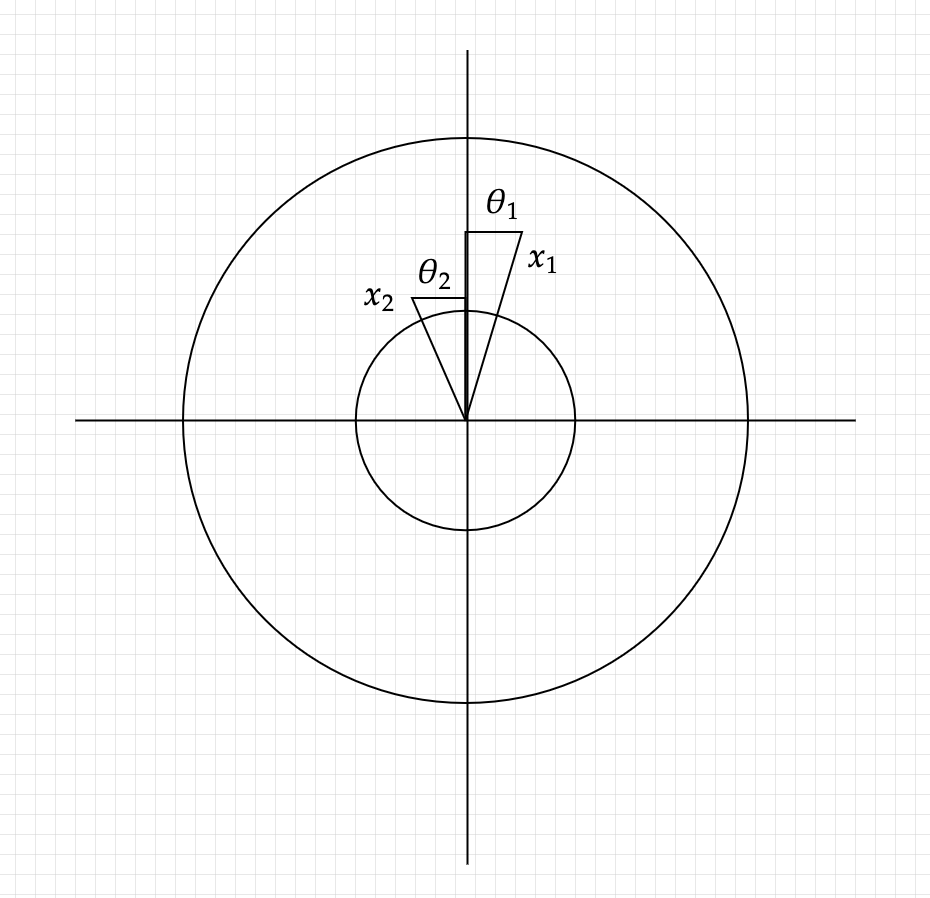
\includegraphics[width=0.3\linewidth]{Chapters/Figures/Screenshot 2025-04-01 at 10.48.42 AM.png}
    \caption{Geometric visualization of the Minkowski sum of two spheres $S^{n-1}(r_1)$ and $S^{n-1}(r_2)$, showing how the resulting set forms a spherical shell with inner radius $r_2-r_1$ and outer radius $r_2+r_1$.}
    \label{fig:sphere-minkowski-sum}
\end{figure}

\noindent This geometric interpretation of the Minkowski sum of spheres is fundamental for understanding the structure of moment-image sets for Hamiltonian $\mathrm{SO}(3)$-spaces. Now, we can classify all possible moment-images of compact connected Hamiltonian $\mathrm{SO}(3)$-spaces as being one of four types: a point (the origin), a sphere, a solid ball, or a spherical shell. \bigskip 

\noindent \textbf{References}: \textcite{Terek2020}

\newpage 
\setcounter{section}{6}

\chapter{Structure of $\rm{SO}(3)$}
\section{Generalizing Delzant to the $\mathrm{SO}(3)$ Case}
Now, let's begin outlining a Delzant correspondence, where the Lie group acting on our manifold is no longer $T^{n}$, but rather $G = \mathrm{SO}(3)$. The key to our approach will be developing several tools:
\begin{enumerate}
    \item Understanding $\mathrm{SO}(3)$ as a composition of shells and rays as in  \textcite{Blaom1996}.
    \item Ultimately, these two points will allow us to build the bundle: $\pi_{\mathcal{O}}: P \to \mathcal{O}$. This allows us to study how a Delzant-type correspondence relates abelian toric actions and nonabelian rotation $\mathrm{SO}(3)$ actions.
\end{enumerate}

First, we would like to establish that $S^{1}$ is the maximum torus of $\rm{SO}(3)$. 

\subsection{Maximal Tori of $\rm{SO}(3)$}

\begin{lemma}[No $2$-Dimensional Subalgebras]
There is no $2$-dimensional Lie-subalgebra of $\mathbb{R}^{3}$
\end{lemma}
\begin{proof}
If $\mathfrak{h}$ is a $2$-dimensional subalgebra of $(\mathbb{R}^{3}, \times)$ and $\{v, w \}$ is a basis for $\mathfrak{h}$ then $v \times w \in \mathfrak{h} \cap \mathfrak{h}^{\perp} = \{0\}$, so $v \times w = 0$ and $\{v, w \}$ is linearly dependent, a contradiction.
\end{proof}

Now, this will be used to prove that: 

\begin{lemma}[Maximal Torus of $\rm{SO}(3)$]
$S^{1}$ is tha maximal torus of $\rm{SO}(3)$
\end{lemma}

\begin{proof}
We note that $(\mathfrak{so}(3), [\cdot, \cdot]) \cong (\mathbb{R}^{3}, \times)$, and that $S^{1}$ is a tori of $\rm{SO}(3)$.Suppose there existed a torus $T$ inside $\rm{SO}(3)$. Then, we find that on the Lie-algebra level, $\mathfrak{t} \subset \mathbb{R}^{2}$ is a $2$-dimensional subalgebra. Contradiction, so $S^{1}$ is the maximum torus of $\rm{SO}(3)$. 
\end{proof}

\noindent \textbf{References:} \textcite{WangZuoqinLieGroups2013}

\subsection{Weyl Chambers and Coadjoint Orbits}

Now, we would like to decompose $\mathfrak{so}(3)$ using spherical coordinates 

\begin{theorem}\label{thm:weyl-chamber-unique}
For each point $\mu_{0} \in \mathfrak{g}_{reg}^{*}$, there passes a unique Weyl chamber. Furthermore, the intersection of an orbit and Weyl chamber is transverse. 
\end{theorem}

\begin{proof}
Equipped with the isomorphism, for each point $p \in (\mathbb{R}^{3}) \setminus \{0\}$, take the line in the dual space passing through $p$. Therefore, Weyl chambers are rays from the origin. The coadjoint orbits are spheres, and it suffices to note that the intersection of a ray and a sphere is transverse. 
\end{proof}

\begin{theorem}\label{thm:weyl-chamber-stabilizer}
If $\mathcal{W}$ is a Weyl chamber in $\mathfrak{g}^{*}$, then $G_{w_{1}} = G_{w_{2}}$, for $w_{1}, w_{2} \in \mathcal{W}$
\end{theorem}

\begin{proof}
Since $w_{1}, w_{2}$ are in the same Weyl chamber, one is a positive scalar multiple of the other. Then, taking exponentials, their stabilizer subgroups are the same. 
\end{proof}

\begin{theorem}\label{thm:spherical-coordinates}
The following is a diffeomorphism:
\begin{equation}
\gamma: \mathbb{R}^{3} \setminus \{0\} \to (0, \infty) \times S^{2}
\end{equation}
\begin{equation}
\gamma(x) = \left( \|x\|, \frac{x}{\|x\|} \right)
\end{equation}
\end{theorem}

\begin{proof}
The diffeomorphism is spherical coordinates taking on $\mathbb{R}^{3}$. To each point we identify a direction and a radius. Therefore, there exists a diffeomorphism between the product of a Weyl chamber and an associated orbit. 
\end{proof}

\noindent \textbf{References:} \textcite{Blaom1996}

\subsection{Moment Maps and Fibre Bundles}
\begin{theorem}\label{thm:stabilizer-dimension}
If $(P, \omega, \mathrm{SO}(3), J)$ is a Hamiltonian $\mathrm{SO}(3)$-space with regular momenta, then $\dim \mathrm{SO}(3)_{x} \leq 1$ for each $x \in P$
\end{theorem}
\begin{proof}
By $\mathrm{SO}(3)$-equivariance of $J$, we know that $dJ_{x}(X_{p}^{\#}(x)) = X^{\#}_{\mathfrak{so}(3)^{\#}}(J(x))$ for all $x \in P$. If $X \in \mathfrak{so}(3)_{x}$, then $X_{P}^{\#}(x) = 0$, and so:
\begin{equation}
X^{\#}_{\mathfrak{so}(3)^{\#}}(J(x)) = 0 \in \mathfrak{so}(3)_{J(x)}
\end{equation}
Now, $\mathfrak{so}(3)_{J(x)}$ cannot have dimension $3$ by the regular momentum assumption, and since $\mathbb{R}^{3}$ does not admit two-dimensional subalgebras, it has dimension less than or equal to $1$:
\begin{equation}
\mathfrak{so}(3)_{x} \subset \mathfrak{so}(3)_{J(x)} \Rightarrow \dim \mathfrak{so}(3)_{x} \leq 1
\end{equation}
\end{proof}

Define the two key projections:

\begin{align}
\pi_{\mathcal{O}}: P \to S^{2}, \; \pi_{\mathcal{O}}(x) = \frac{J(x)}{\|J(x)\|} && \pi_{\mathcal{W}}: P \to \mathbb{R}^{+}, \; \pi_{\mathcal{W}}(x) = \|J(x)\|
\end{align}

\begin{lemma}
$\pi = \pi_{\mathcal{O}}$ is surjective
\end{lemma}

\begin{proof}
Since the momentum image is not trivial, there exists elements $g \in G$, $w \in \mathcal{W}$, and $x \in P$ such that $J(x) = g \cdot w$, where $J$ is the momentum map. This implies that $G \cdot w \in \operatorname{Im}(J)$. Now, we note that $\pi_{\mathcal{O}}$ maps each coadjoint orbit diffeomorphically onto $\mathcal{O}$. Therefore: there exists $h \in G \cdot w$ such that $\pi_{\mathcal{O}} (h) = \mu$. Furthermore, there exists $x' \in P$ such that $J(x') = \nu$. This proves that $\pi_{\mathcal{O}} \circ J$ is surjective.
\end{proof}

\begin{theorem}
$\pi^{-1}(\mu)$ is a fibre bundle $P \to \mathcal{O}$:
\end{theorem}

\begin{proof}
We can verify that the differential map $d\pi_{\mathcal{O}}|_{J(x)} \circ dJ_x$ is surjective. Therefore, each fibre $\pi^{-1}(\mu)$ forms a submanifold of $P$. Now, we must construct local trivializations to complete the proof. Consider a point $\mu_0 \in \mathcal{O}$ and its isotropy subgroup $G_{\mu_0}$. For any neighborhood $U$ of $\mu_0$, we construct a $G_{\mu_0}$-invariant neighborhood:
\begin{equation}
U' = \bigcup_{h \in G_{\mu_0}} h(U)
\end{equation}
Since the actions of $G$ by left multiplication and its inverse are continuous, the following sets are open:
\begin{align}
U_1' &= \bigcup_{g \in G} g \cdot U'\\
U_2' &= \bigcup_{g \in G} g^{-1} \cdot U'
\end{align}
Taking the intersection $U = U_1' \cap U_2'$, we obtain a neighborhood with two important properties:
\begin{enumerate}
\item $U$ is $G_{\mu_0}$-invariant
\item If $g \cdot \mu_0 \in U$, then $g^{-1} \cdot \mu_0 \in U$
\end{enumerate}
Now, choose $s$ to be a local section of the principal $G_{\mu_0}$-bundle $G \to G/G_{\mu_0}$ such that:
\begin{equation}
s(g G_{\mu_0}) = g
\end{equation}
Also, define the diffeomorphism:
\begin{equation}
\phi_{\mu_0}(g G_{\mu_0}) = g \cdot \mu_0
\end{equation}

\noindent The map $\psi: U \times F \to \pi^{-1}(U)$ defined by:
\begin{equation}
\psi(\mu, x) = s(\phi^{-1}_{\mu_0}(\mu)) \cdot x
\end{equation}
is a local bundle chart, where $F$ denotes the fibre. First, we verify that $\psi$ maps correctly by examining its composition with $\pi$:
\begin{equation}
\pi(\psi(\mu, x)) = \pi(s(\phi_{\mu_0}^{-1}(\mu)) \cdot x) = \phi_{\mu_0}(\phi_{\mu_0}^{-1}(\mu)) = \mu
\end{equation}
This shows that $\psi$ preserves the fibres of $\pi$. Next, we show that $\psi$ is well-defined and invertible. For any $y \in \pi^{-1}(U)$:
\begin{equation}
\psi(\psi^{-1}(y)) = s \circ \phi^{-1}_{\mu_0} \circ \pi \circ \phi_{\mu_0} \circ s^{-1}(y) = y
\end{equation}
Since both $\psi$ and $\psi^{-1}$ are smooth maps, we conclude that $\psi$ is a diffeomorphism and thus a local bundle chart. The inverse map can be expressed as:
\begin{equation}
\psi^{-1}(y) = (\pi(y), (s(\phi_{\mu_0}^{-1}(\pi(y))))^{-1} \cdot y)
\end{equation}

\noindent The local charts for our bundle are:
\begin{equation}
U_{\mu} = \{g \cdot U: g \in \phi_{\mu_0}^{-1}(\mu) \}
\end{equation}
Recall that $\phi_{\mu_0}^{-1}(\mu) = g G_{\mu_0}$ corresponds to elements satisfying $g \cdot \mu_0 = \mu$. Since $\mathcal{O}$ is compact, we can extract a finite subcover $\{U_{\mu_k}\}_{k=1}^n$ of these sets.
For each $k$, we define the local trivialization:
\begin{equation}
\psi_k: U_{\mu_k} \times F \to \pi^{-1}(U_{\mu_k})
\end{equation}
\begin{equation}
\psi_k(\mu, x) = g_k \cdot \psi(g_k^{-1} \cdot \mu, x)
\end{equation}
where $g_k \in G$ satisfies $g_k \cdot \mu_0 = \mu_k$. The transition functions between overlapping charts are:
\begin{align}
\psi_j^{-1} \circ \psi_k&: (U_{\mu_j} \cap U_{\mu_k}) \times F \to (U_{\mu_j} \cap U_{\mu_k}) \times F\\
\psi_j^{-1} \circ \psi_k(\mu, x) &= (\mu, g_j^{-1} g_k \cdot x)
\end{align}
These transition functions take values in a subgroup of the maximal torus $T$, which completes the proof that $\pi: P \to \mathcal{O}$ is a fibre bundle with structure group contained in $T$.
\end{proof}

\begin{theorem}[\textcite{Blaom1996}] \label{thm:fibre-bundle}
$\pi: P \to \mathcal{O}$ is a fibre bundle, with the structure group of the bundle being a subgroup of the maximal torus, $T$. 
\end{theorem}

\subsection{Symplectic Properties of Moment Maps}
\begin{theorem}[Guillemin and Sternberg]\label{thm:transverse-symplectic}
Let $Z$ be a submanifold of $\mathfrak{g}^*$ such that $J$ is transverse to $Z$ and:
$T_{z} Z \oplus T_{z}(G \cdot z) = \mathfrak{g}^* $. Then $J^{-1}(Z)$ is a symplectic submanifold of $P$. 
\end{theorem}

\begin{lemma}
By equivariance, $dJ_{x}$ spans the tangent space to a coadjoint orbit $\mathcal{O}$. Since $Z = \mathcal{W}$ is transverse to $\mathcal{O}$, it follows that $dJ_{x}$ intersects $\mathcal{W}$ transversely, and we can apply Theorem \ref{thm:transverse-symplectic} to $Z = \mathcal{W}$, to find that: $J^{-1}(\mathcal{W})$ is a symplectic submanifold. Note that fibres of $\pi: P \to \mathcal{O}$ are just $J^{-1}(\mathcal{W})$. Therefore, using the symplectic form on each submanifold, we have a smoothly varying choice of vector spaces $V_{x} = \operatorname{Ker} d \pi_{x}$: $T_{x} P \cong V_{x} \oplus V_{x}^{\omega}$
\noindent This can be phrased as there exists a projection map: $\beta: TP \to \ker d\pi_{x} $
  
\end{lemma}

\begin{theorem}[{\cite{Blaom1996}}]\label{thm:kernel-moment-map}
Let $v \in \operatorname{Ker} dJ_{x}$. Then $v \in \left[ T_{x} J(G \cdot x) \right]^{\omega}$.
\end{theorem}

\begin{proof}
The result follows from the identity
\begin{equation}
dJ_{x}(w) = \omega(\xi, w), \quad \xi \in T_{x} J(G \cdot x). 
\end{equation}
\end{proof}

\begin{theorem}\label{thm:horizontal-tangent}
The horizontal subspace satisfies
\begin{equation}
\operatorname{Hor}_{x} \subset T_{x}(G \cdot x).
\end{equation}
\end{theorem}

\begin{proof}
Recall that $\operatorname{Hor}_{x} = \ker d\pi_{x}$. Since $\operatorname{Ker} dJ_{x} \subset \operatorname{Ker} d\pi_{x}$, we have $\operatorname{Ker} dJ_{x} \subset \operatorname{Hor}_{x}$. By Theorem~\ref{thm:kernel-moment-map}, we obtain $\operatorname{Hor}_{x} \subset T_{x}(G \cdot x)$.
\end{proof}

\begin{theorem}\label{thm:map-onto-horizontal}
The fundamental vector field map $\xi \mapsto \xi_{P}$ maps $\mathfrak{t}^{-}$ onto $\operatorname{Hor}_{x}$.
\end{theorem}

\begin{proof}
By Theorem~\ref{thm:horizontal-tangent}, it suffices to establish injectivity, i.e., $\mathfrak{g}_{x} \cap \mathfrak{t}^{-} = \{0\}$. This follows immediately from the fact that $\mathfrak{g}_{x} = \mathfrak{t}$.
\end{proof}

\begin{theorem}\label{thm:derivative-moment-map}
The differential of the momentum map $dJ_{x}$ sends 
\begin{align}
\operatorname{Hor}_{x} \text{ to } T_{J(x)}(G \cdot J(x)) \cong \underline{\mathfrak{t}}^{-} \subset \mathfrak{g}^{*}
\end{align}

\end{theorem}

\begin{proof}
We need to show that $\operatorname{Hor}_{x} \cap \operatorname{Ker} dJ_{x} = \{0\}$. Since 

\begin{align}
\operatorname{Ker} dJ_{x} \subset \operatorname{Ker} d\pi_{x} && \operatorname{Hor}_{x} \cap \operatorname{Ver}_{x} = \{0\}
\end{align}

\noindent the result follows.
\end{proof}

\begin{theorem}\label{thm:symplectic-pairing}
For any $\xi, \nu \in \mathfrak{g}$, the symplectic form satisfies
\begin{equation}
\omega(\xi_{P}(x), \nu_{P}(x)) = \langle J(x), [\xi, \nu] \rangle,
\end{equation}
where $\langle \cdot, \cdot \rangle$ denotes the canonical pairing between $\mathfrak{g}^*$ and $\mathfrak{g}$.
\end{theorem}

\begin{proof}
The following computation yields the necessary result:
\begin{equation}
\omega(\xi_{P}(x), \nu_{P}(x)) = \omega(X_{J_{\xi}}(x), X_{J_{\nu}}(x)) = J_{[\xi, \nu]}(x) = \langle J(x), [\xi, \nu] \rangle. \qedhere
\end{equation}
\end{proof}

\begin{remark}
Theorem~\ref{thm:symplectic-pairing} establishes the fundamental relationship between the symplectic structure on $P$ and the Lie algebra structure of $\mathfrak{so}(3)$, completing the generalization of Delzant's correspondence to the $\mathrm{SO}(3)$ case described in \textcite{Blaom1996}
\end{remark} \bigskip

\noindent \textbf{References:} \textcite{Blaom1996}

\newpage 
\setcounter{section}{7}

\chapter{$T$-Actions and Further Generalizations}
\section{Canonical T-Action and Generalization of Delzant's Theorem}

In this last section, we were studying the fibre  $\pi: P \to \mathcal{O}$, and we noted that the transition functions between fibres were contained in a fundamental torus $G_{\mu}$. Now, we want to use this fact to develop an $S^{1}$-action on fibres. This twisted $S^{1}$-action will allow us to develop a Delzant-type correspondence, where when we compare two manifolds, if the $S^{1}$-spaces arising via bundle fibres are symplectomorphic via the twisted $S^{1}$-action, then the corresponding Hamiltonian $\mathrm{SO}(3)$-spaces are equivariant symplectomorphic. In this section, we will:
\begin{enumerate}
    \item Develop a framework for the twisted $S^{1}$-action.
    \item Prove a version of Delzant's Theorem.
\end{enumerate}
\subsection{Construction of the Twisted $S^1$-Action}
Recall how the transition functions arising from the $\pi$ bundle acted. On each fibre $\pi^{-1}(\mu)$ there is the group action $G_{\mu}$. Now, we consider the group isomorphism:
\begin{align}
k_{\mu}: S^{1} \to G_{\mu} \text{ where } \mu = g \cdot \mu_{0} && \text{ given by } k_{\mu}(t) \mapsto gtg^{-1} 
\end{align}

\noindent This allows us to define an $T$-action $\bullet$ on $P$ given by: 

\begin{defn}[$T$-action on $P$]
Let $(P, \omega, \rm{SO}(3))$ be a symplectic manifold with Hamilitonian Lie action. Then, a twisted $T$ action $T \circlearrowleft P$ is given by:

\begin{equation}
t \bullet x = k_{\pi(x)}(t) \cdot x
\end{equation}

\noindent Where $k_{\mu}(t) \mapsto gtg^{-1}$, and $T$ is the maximum tori of $\rm{SO}(3)$.
\end{defn}

\begin{remark}
We say that $T$ acts on $x$ via a twisted action $k_{\pi(x)}$, which is manifestly abelian. By definition, the generators of this action are:
\end{remark}

\begin{defn}[Infinitesimal generators of $T$ action]
The infinitesimal generators are:

\begin{equation}
\xi_{P} = \lim_{\tau \to 0} \frac{d}{d \tau} \exp(\tau \xi) \bullet x
\end{equation}
\end{defn}

\begin{lemma}[Generators of $T$-action]
The infinitesimal generators of $T = S^{1}$ and $G = \mathrm{SO}(3)$ are related for any $\xi \in \mathfrak{t} \subset \mathfrak{g}$ by:
\begin{equation}
\xi_{P}^{T}(x) = (\mathrm{Ad}_{g} \xi)_{P} (x)
\end{equation}
\end{lemma}

\begin{proof}
This follows by derivation of the above $\bullet$ definition. Take the derivative of $\exp(t \xi) \cdot x$:
\begin{align}
\xi_{P}^{T} &= \lim_{\tau \to 0} \frac{d}{d \tau} g \exp(\tau \xi) g^{-1}\\
\xi_{P}^{T} &= \mathrm{Ad}_{g} \xi
\end{align}
Where $\mu = g \cdot \mu_{0}$, or $\pi(x) = g \cdot \mu_{0} \Longleftrightarrow g^{-1} \cdot x \in \pi^{-1}(\mu_{0})$.
\end{proof}

\begin{theorem}[\textcite{Blaom1996}]\label{thm:t-action-hamiltonian}
The $T$ action defined above is Hamiltonian. Furthermore, a $T$-equivariant moment map for this action is $j = i \circ \pi_{\mathcal{W}} \circ J$ 
\end{theorem}

\begin{proof}
We want to show:
\begin{equation}
\langle dj_{x'} v, \xi \rangle = \langle dJ_{x'} v, \mathrm{Ad}_{g} \xi \rangle
\end{equation}
when $v \in \operatorname{Hor}_{x}$ and when $v \in T_{x} \pi^{-1}(\mu)$. As these are $\omega$-orthogonal, that will imply that:
\begin{equation}
\langle dj_{x'} v, \xi \rangle = \langle dJ_{x'} v, \mathrm{Ad}_{g} \xi \rangle
\end{equation}
everywhere. Moreover, this will prove that $T$ is Hamiltonian with the infinitesimal generators:
\begin{equation}
X_{j_{\xi}} = \xi_{P}^{T}(x)
\end{equation}
Let's prove the first part - note that $j$ is $G$-invariant, since orbits factor out under $\pi_{\mathcal{W}}$. Since the $T \trianglelefteq G$ action is trivial, we also have $j$ is $T$-equivariant. For fixed $\mu_{0}$, choose $\mu = \pi(x) = g \cdot \mu_{0}$, and note that for the Weyl chamber $\mathcal{W}$, $g^{-1} J(x') \in \mathcal{W}$. Now, for any $\xi \in \mathfrak{t}$, we note that $g^{-1} J(x')$ survives the projection $\pi_{\mathcal{W}}$. 
\begin{equation}
\langle j(x'), \xi \rangle = \langle \pi_{\mathcal{W}} J(x'), \xi \rangle = \langle g^{-1} \cdot J(x'), \xi \rangle
\end{equation}
Taking derivatives of both sides, we have:
\begin{equation}
\langle dj_{x'} v, \xi \rangle = \langle dJ_{x'} v, \mathrm{Ad}_{g} \xi \rangle
\end{equation}
In particular, this occurs when $x' \in T_{x} \pi^{-1}(\mu)$.
\end{proof}
\begin{lemma}\label{lem:derivatives-vanish}
Both the derivative of $j$ and the derivative of $J$ vanish on horizontal fibres:
\begin{equation}
\{\langle dJ_{x'} v, \mathrm{Ad}_{g} \xi \rangle: v \in \operatorname{Hor}_{x} \} = 0
\end{equation}
\end{lemma}
\begin{proof}
Firstly, since $j$ is $G$-invariant, yet elements of $\operatorname{Hor}_{x}$ live in the domain $T_{x}(G \cdot x)$, we conclude that $\{\langle dj_{x'} v, \xi \rangle: v \in \operatorname{Hor}_{x} \} = 0$. Now, to show that the derivative of $J$ vanishes, note that $dJ_{x'} v$ must be tangent to the coadjoint orbit through $x$, so that:
$dJ_{x'} v = \mathrm{ad}_{\nu} J(x')$. Then:
\begin{align}
\langle dJ_{x'} v, \mathrm{Ad}_{g} \xi \rangle &= \langle \mathrm{ad}_{\nu} J(x'), \mathrm{Ad}_{g} \xi \rangle\\
&= \langle J(x'), [\nu, \mathrm{Ad}_{g} \xi] \rangle\\
&= \langle \mathrm{Ad}_{g}^{*} J(x'), [\mathrm{Ad}_{g^{-1}} \nu, \xi] \rangle\\
&= -\langle \mathrm{ad}^{*}_{\xi} \left[ g^{-1} \cdot J(x') \right], \mathrm{Ad}_{g^{-1}} \nu \rangle
\end{align}
Since $g^{-1} J(x') \in \mathcal{W}$, $\mathrm{ad}^{*}_{\xi} \left[ g^{-1} \cdot J(x') \right] = 0$, the conclusion follows.
\end{proof}
\begin{lemma}[Classical] \label{lem:local-sections}
If $G$ is a Lie group and $H$ a closed subgroup of $G$, then $G \to G/H$ is a principal $G$ bundle.
\end{lemma}
We will use this lemma to build charts for a symplectomorphism on the $G = \mathrm{SO}(3)$ level between manifolds. 

\noindent \textbf{References}: \textcite{Blaom1996}

\subsection{Equivalence of Hamiltonian G-Spaces}
\begin{theorem}\label{thm:hamiltonian-g-spaces-equivalence}
Let $G$ be a compact, connected Lie group. Then two Hamiltonian $G = \rm{SO}(3)$-spaces with regular momenta are equivalent if and only if their associated $T$-spaces are equivalent.
\end{theorem}
\begin{proof}
The forward direction is clear. Let $(P_{1}, \omega_{1}, G, J^{1})$ and $(P_{2}, \omega_{2}, G, J^{2})$ be Hamiltonian $G$-spaces. We have symplectic fibrations $\pi_{1}: P_{1} \to \mathcal{O}$ and $\pi_{2}: P_{2} \to \mathcal{O}$. Let $F_{1}$ and $F_{2}$ be fibres of $\pi_{1}$ and $\pi_{2}$ over $\mu_{0}$ respectively, where $\mu_{0}$ is just a choice $\mu_{0} \in \mathfrak{g}_{reg}^{*}$. Let's assume we have a $T$-equivariant symplectomorphism:
\begin{align}
\varphi&: F_{1} \to F_{2}\\
J^{F_{2}} \circ \varphi &= J^{F_{1}}
\end{align}
Let $x \in P_{1}$ such that $\pi_{1}(x) = g \cdot \mu_{0}$. Define:
\begin{equation}
\phi(x) = g \cdot \varphi(g^{-1} \cdot x)
\end{equation}

\begin{figure}
    \centering
    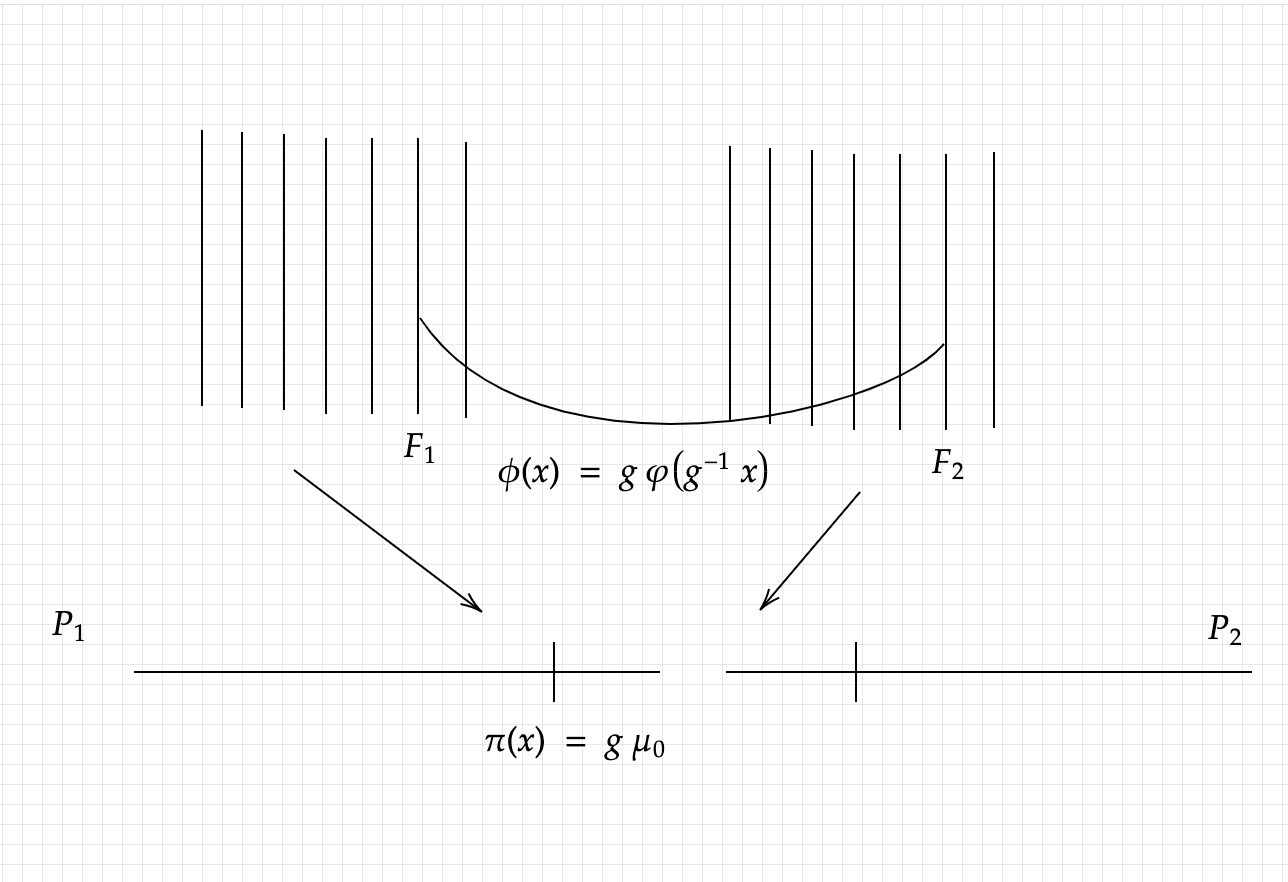
\includegraphics[width=0.5\linewidth]{Chapters/Figures/w.png}
    \caption{To move between fibres, we define $\phi(x) = g \cdot \varphi(g^{-1} \cdot x) $} 
    \label{fig:enter-label}
\end{figure}


\noindent It suffices to show that $\phi$ is well-defined, $\phi$ is $G$-equivariant and $J^{2} \circ \phi = J^{1}$, and there exists an inverse for $\phi$.
\end{proof}
\begin{lemma}\label{lem:phi-well-defined}
$\phi(x)$ is well defined, for a choice of $g \in G$.
\end{lemma}
\begin{proof}
We consider $g$ such that $g \cdot \mu_{0} = \mu_{0}$. Note that $g \cdot \mu_{0}$ is unique up to a factor of $g \cdot t$, where $t \in G_{\mu_{0}}$. Now we note that $\phi(x)$ does not depend on $g$:
\begin{align}
\phi(x) &= gt \cdot \varphi(t^{-1} \circ g^{-1} \cdot x)\\
\phi(x) &= g \cdot \varphi(g^{-1} \cdot x)
\end{align}
\end{proof}
\begin{lemma}\label{lem:phi-equivariant}
$\phi$ is $G$-equivariant. 
\end{lemma}
\begin{proof}
Since $\pi_{1}(x) = g \cdot \mu_{0}$, $\pi_{1}(h \cdot x) = hg \cdot \mu_{0}$ by equivariance. Now: 
\begin{equation}
\phi(h \cdot x) = hg \cdot \varphi(g^{-1} h^{-1} \cdot h x) = h \cdot \phi(x)
\end{equation} \end{proof}
\begin{lemma}\label{lem:moment-maps-agree}
$J^{F_{2}} \circ \varphi = J^{F_{1}}$ implies that $J^{2} \circ \phi = J^{1}$.
\end{lemma}
\begin{proof}
We do the following computation: \begin{align}
(J^{2} \circ \phi)(x) &= J^{2}(g \cdot \varphi(g^{-1} \cdot x))\\
&= g \cdot J^{F_{2}}(\varphi(g^{-1} \cdot x))\\
&= g \cdot J^{F_{1}}(g^{-1} \cdot x)\\
&= J^{1}(x)
\end{align}
\end{proof}
\begin{lemma}\label{lem:phi-inverse}
There exists an inverse, $\phi^{-1}$ for $\phi$. 
\end{lemma}
\begin{proof}
This follows by symmetry of definitions:
\begin{equation}
\phi^{-1}(y) = g \cdot \varphi^{-1}(g^{-1} \cdot y)
\end{equation}
Note that:
\begin{equation}
\phi^{-1}(\phi(x)) = g \cdot \varphi^{-1}(g^{-1} \cdot g \cdot \varphi(g^{-1} \cdot x)) = x
\end{equation}
\end{proof}
Now, by hypothesis:
\begin{equation}
\varphi: F_{1} \to F_{2}
\end{equation}
\noindent is a symplectic diffeomorphism of two fibres over $\mu_{0}$. Equivalently, this is a diffeomorphism of the kernel of $d \pi_{1}$ and $d \pi_{2}$ around points $x \in P_{1}, \; \varphi(x) \in P_{2}$:
\begin{equation}
\varphi: \ker (d\pi_{1})_{x} \to \ker (d\pi_{2})_{\varphi(x)}
\end{equation}

\noindent Since $\operatorname{Hor}_{\phi(x)}^{2} = (d\pi_{2})_{\varphi(x)}^{\omega}$, and $\operatorname{Hor}_{x}^{1} = (d\pi_{1})_{x}^{\omega}$, it follows $d\phi$ maps $\operatorname{Hor}_{x}^{1}$ to $\operatorname{Hor}_{\phi(x)}^{2}$. Furthermore, since each is the $\omega$-complement, the isomorphism is symplectic. So, $\phi$ is a symplectic diffeomorphism. 

\noindent \textbf{References}: \textcite{Blaom1996}

\subsection{Delzant Correspondence for $\mathrm{SO}(3)$}
\begin{theorem}[\textcite{Delzant1988, Blaom1996}] \label{thm:delzant-so3}
Consider two $4$-dimensional, compact Hamilitonian $\rm{SO}(3)$ spaces $(P_{1}, \omega_{1}, \mathrm{SO}(3), J^{1})$ and $(P_{2}, \omega_{2}, \mathrm{SO}(3), J^{2})$ whose moment images do not contain $0$. Denote $S = S^{1}_{xy}$ the circle in the $xy$-plane. If rotation actions in $S$ are faithful on $(J^{i})^{-1}(\hat{z})$ then the spaces are equivalent up to equivariant symplectomorphism. 
\end{theorem}


\begin{figure}[htbp]
    \centering
    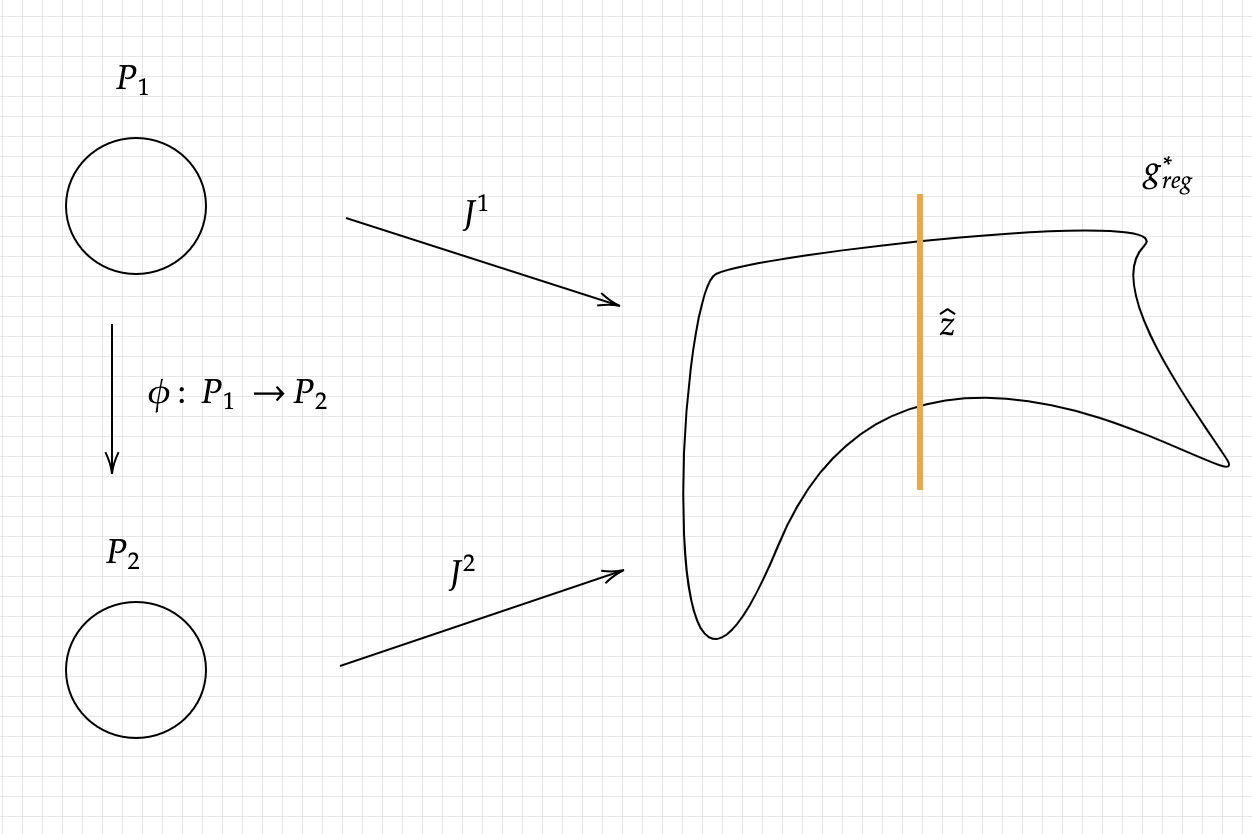
\includegraphics[width=0.4\linewidth]{Chapters/Figures/Screenshot 2025-03-07 at 1.40.07 PM.png}
    \caption{Existence of a $\mathrm{SO}(3)$-equivariant symplectomorphism $\phi$ comes from agreement of two moment maps, $J^{2}$ and $J^{1}$, such that the inverse images of $\hat{z}$ are acted on faithfully.}
    \label{fig:so3-symplectomorphism}
\end{figure}

\begin{proof}
Let $(P_{1}, \omega_{1}, \mathrm{SO}(3), J^{1})$ and $(P_{2}, \omega_{2}, \mathrm{SO}(3), J^{2})$ be two $4$-dimensional, compact Hamiltonian $\mathrm{SO}(3)$ spaces whose moment-images do not contain $0$. Let $F_{1}$ be a fibre of $\pi_{1}$. Then $\dim F_{1} + \dim \mathcal{O} = \dim P_{1}$ and $\dim F_{2} + \dim \mathcal{O} = \dim P_{2}$. By Delzant's Theorem, we have that that $\dim F_{1} = 2 \dim S^{1} = 2$. Furthermore, $\dim \mathcal{O} = 2$. Therefore, we require that $\dim P_{1} = \dim P_{2} = 4$. By \textit{Delzant's Theorem}, because both $S^{1}$ rotation actions are faithful with respect to the twisted action, the Delzant spaces $S^{1} \circlearrowright P_{1}$ and $S^{1} \circlearrowright P_{2}$ are symplectomorphic. By Theorem \ref{thm:hamiltonian-g-spaces-equivalence}, the $\mathrm{SO}(3)$ spaces are equivalent up to equivariant symplectomorphism by an element of $\mathrm{SO}(3)$. 
\end{proof} \bigskip 

\textbf{References}: \textcite{Delzant1988, Blaom1996}



\chapter{Necessity of Regular Momenta}
\section{Necessity of the Regular Condition}
Let's study the theorem in the restriction when the image of $J$ is no longer regular. Using the Fubini-Study metric, we are able to find the image of the moment map $J$, arising from the Lie group action of $\mathrm{SO}(3)$ on $(\mathbb{C}P^{2}, \omega_{FS})$, and study the unique properties of this construction.

\subsection{Fubini-Study Metric and Symplectic Structure}

To develop this construction, let $V$ be a complex vector space, with dimension $\dim_{\mathbb{C}} V = n+1$ with a Hermitian inner product $\langle \cdot, \cdot \rangle$ and $\pi: V \setminus \{0\} \to \mathbb{P}V$. 

\begin{lemma}[Symplectic form on $V$]
$V$ is a vector space with symplectic form $\Omega(v,w) = \Im \langle v, w \rangle$
\end{lemma}

\begin{proof}
We verify that $\Omega$ is skew-symmetric:
\begin{equation}
\Omega(w, v) = \Im \langle w, v \rangle = \Im \overline{\langle v, w \rangle} = - \Im \langle v, w \rangle = - \Omega(v,w)
\end{equation}
Where we use conjugate symmetry to get that $\langle v, w \rangle = \overline{\langle w, v \rangle}$. Replacing $w$ with $iw$, this form is also non-degenerate since if $\Omega(v, \cdot) = 0$, then $\Im \langle v, w \rangle = 0$ and for choices of $iw$, $\Re \langle v, w \rangle = 0$ as well, showing that $v = 0$ using that $\langle \cdot, \cdot \rangle$ is non-degenerate.
\end{proof}

\begin{remark}
Now, we want to find a symplectic form $\omega_{FS}$ for $(\mathbb{P} V, \omega_{FS})$
\end{remark}

Note that in the construction $\pi: V \setminus \{0\} \to \mathbb{P} V$, orthogonal complements survive in the projectivization: $d\pi_{v}$ maps $(\mathbb{C} v)^{\perp}$ isomorphically onto $T_{\pi(v)} \mathbb{P}V$. Therefore, we work backwards, and consider a symplectic built from the orthogonal complements of $\xi_{1}, \xi_{2}$ with respect to $v$ on $V$. These are $\xi_{i} - \frac{\langle \xi_{i}, v \rangle}{\langle v, v \rangle}v \in (\mathbb{C} v)^{\perp}$ for $i \in \{1,2 \}$. 

\begin{remark}
Therefore, we suspect that $$\omega_{v}(\zeta_{1}, \zeta_{2}) = \Im \left\langle \xi_{1} - \frac{\langle \xi_{1}, v \rangle}{\langle v, v \rangle}v, \xi_{2} - \frac{\langle \xi_{2}, v \rangle}{\langle v, v \rangle}v \right\rangle$$ would be a symplectic form for $\mathbb{P} V$. However, this form doesn't yet survive in the quotient. Consider the diffeomorphism given by $m_{\lambda}: V \setminus \{0\} \to V \setminus \{0\}$ given by $m_{\lambda}(v) = \lambda v$. We note that we need $m_{\lambda}^{*} \omega = \omega$. Yet, observe that: $m_{\lambda}^{*} \omega_v = |\lambda|^2 \omega_{v}(\zeta_{1}, \zeta_{2})$. It suffices to take the Fubini-Study metric to be a normalized $\frac{1}{\langle v, v \rangle}$ expression of the proposed two-form. The reason for this normalization is that $\langle \lambda v, \lambda v \rangle$ cancels out the $|\lambda|^2$ term.
\end{remark}


\begin{lemma}[Symplectic form on $\mathbb{P} V$]
$(\mathbb{P} V, \omega_{FS})$ is a symplectic manifold with:
\begin{equation}
\left( \omega_{FS} \right)_{[v]}(\zeta_{1}, \zeta_{2}) = \frac{1}{\langle v, v \rangle} \Im \left\langle \xi_{1} - \frac{\langle \xi_{1}, v \rangle}{\langle v, v \rangle}v, \xi_{2} - \frac{\langle \xi_{2}, v \rangle}{\langle v, v \rangle}v \right\rangle 
\end{equation}
\noindent where $\xi_{j} \in V$ are such that $d \pi_{v} \xi_{j} = \zeta_{j}$
\end{lemma}

Now note that $\omega_{FS}$ is well defined and, mimicking the above argument, it is non-degenerate, while closedness follows from $PU(V, \langle \cdot, \cdot \rangle)$ invariance according to \textcite{Arnold2010}. \bigskip 

\noindent \textbf{References}: \textcite{Arnold2010}

\subsection{Moment Map for Unitary Representations}
We are now able to apply Proposition 1.1 in \textcite{Wildberger1992}. 

\begin{lemma}[\textcite{Wildberger1992}]
If $G \to U(V, \langle \cdot, \cdot \rangle)$ is a unitary representation of a Lie group $G$, the induced action of $G$ on $\mathbb{P}V$ is Hamiltonian, with moment map: 
\begin{equation}
J^{X}([v]) = \frac{1}{2i} \frac{\langle X \cdot v, v \rangle}{\langle v, v \rangle}
\end{equation}
\noindent for \([v] \in \mathbb{P}V\) and \(X \in \mathfrak{g}\).
\end{lemma}

\noindent \textbf{References}: \textcite{Wildberger1992}

\subsection{Moment Map for $\mathrm{SO}(3)$ Action on $\mathbb{C}P^2$}
Now, consider the action of $G = \mathrm{SO}(3)$ on $V = \mathbb{C}^{3}$ given by evaluations, that is: $A \cdot z = Az$, where $A$ is the $\mathbb{C}$-linear extension of $A: \mathbb{R}^{3} \to \mathbb{R}^{3}$. In other words, we compose with the inclusion $\mathrm{SO}(3)$ into $\mathrm{SU}(3)$. The Hermitian inner product in $\mathbb{C}^{3}$ is:
\begin{equation}
\langle (z_{1}, z_{2}, z_{3}), (w_{1}, w_{2}, w_{3}) \rangle = z_{1} \overline{w_{1}} + z_{2} \overline{w_{2}} + z_{3} \overline{w_{3}}
\end{equation}
Now, we compute the moment image of the Hamiltonian action of $\mathrm{SO}(3)$ on $(\mathbb{C}P^{2}, \omega_{FS})$. With the usual identification of $\mathfrak{so}(3)^{*} \cong \mathbb{R}^{3}$ we note that $J: \mathbb{C}P^{2} \to \mathbb{R}^{3}$.
We want to use the moment map formula to compute the moment-image of the resulting Hamiltonian action 
of $\mathrm{SO}(3)$ on $(\mathbb{C}P^2,\omega_{\mathrm{FS}})$ \textcite{Wildberger1992}. 
With the usual identification of $\mathfrak{so}(3)^*$ with $\mathbb{R}^3$ in place.

\begin{lemma}[Moment Map $\mu$ for $\mathbb{C} P^{2}$]
We claim the moment map $\mu$ is:

\begin{equation}
\mu \bigl([z_1 : z_2 : z_3]\bigr) = 
\left(
\frac{\mathrm{Im}(z_2 \overline{z_3})}{|z_1|^2 + |z_2|^2 + |z_3|^2},\;
\frac{\mathrm{Im}(z_3 \overline{z_1})}{|z_1|^2 + |z_2|^2 + |z_3|^2},\;
\frac{\mathrm{Im}(z_1 \overline{z_2})}{|z_1|^2 + |z_2|^2 + |z_3|^2}
\right).
\end{equation}
    
\end{lemma}

\begin{proof}
The following are bases on $\mathfrak{so}(3)^{*}$ with the usual identification:
\begin{equation}
E_1 =
\begin{pmatrix}
0 & 0 & 0 \\
0 & 0 & -1 \\
0 & 1 & 0
\end{pmatrix},
\quad
E_2 =
\begin{pmatrix}
0 & 0 & 1 \\
0 & 0 & 0 \\
-1 & 0 & 0
\end{pmatrix},
\quad
E_3 =
\begin{pmatrix}
0 & -1 & 0 \\
1 & 0 & 0 \\
0 & 0 & 0
\end{pmatrix}.
\end{equation}
To show the formula for the moment map, we apply Wildberger's formula to each of the basis elements and use linearity: 
\begin{equation}
E_1 z =
\begin{pmatrix}
0 & 0 & 0 \\
0 & 0 & -1 \\
0 & 1 & 0
\end{pmatrix}
\begin{pmatrix}
z_1 \\[6pt]
z_2 \\[6pt]
z_3
\end{pmatrix}
=
\begin{pmatrix}
0 \\ -z_3 \\ z_2
\end{pmatrix},
\end{equation}
so that
\begin{align}
\frac{1}{2i}\,\frac{\langle E_1 z,\,z\rangle}{\langle z,\,z\rangle}
&=
\frac{1}{2i}
\frac{\bigl(-\,z_3\,\overline{z_2} + z_2\,\overline{z_3}\bigr)}%
     {|z_1|^2 + |z_2|^2 + |z_3|^2} \\&=
\frac{1}{2i}\,\frac{2\,i\,\mathrm{Im}(z_2 \overline{z_3})}{|z_1|^2 + |z_2|^2 + |z_3|^2} =
\frac{\mathrm{Im}(z_2 \overline{z_3})}{|z_1|^2 + |z_2|^2 + |z_3|^2}.
\end{align}
Similarly, we have that
\begin{equation}
\frac{1}{2i}\,\frac{\langle E_2 z,\,z\rangle}{\langle z,\,z\rangle} =
\frac{\mathrm{Im}(z_3 \overline{z_1})}{|z_1|^2 + |z_2|^2 + |z_3|^2}
\quad\text{and}\quad
\frac{1}{2i}\,\frac{\langle E_3 z,\,z\rangle}{\langle z,\,z\rangle} =
\frac{\mathrm{Im}(z_1 \overline{z_2})}{|z_1|^2 + |z_2|^2 + |z_3|^2}.
\end{equation}
\end{proof}

\subsection{Significance for Delzant Correspondence}

\begin{remark}
Therefore, our formula for the moment map holds. Yet, the action does not have regular momenta, since $\mu([0:0:1]) = (0,0,0)$ is the origin. As we have proven, this means that the image of $J$ is a closed ball. Furthermore, as we will see below, another space which has the closed ball as its moment map image is $S^{2}(r) \times S^{2}(r)$. Therefore, we see that regular momenta is a necessary assumption in the statement of our theorem. Without it, we would have concluded that $S^{2}(r) \times S^{2}(r) \cong \mathbb{C}P^2$. But this is impossible, as the cohomology is wrong: $H^2_{dR}(\mathbb{C}P^2) = \mathbb{R}$ while $H^2_{dR}(S^2 \times S^2) = \mathbb{R}^2$.
\end{remark}



\newpage

\setcounter{section}{9}

\chapter{Classification of Hamilitonian $\rm{SO}(3)$-actions}
\section{Action Classification and Realization Theorems}
In general, we can realize each of the four prototypes, and therefore, we have a classification theorem for spaces admitting effective, Hamiltonian $\mathrm{SO}(3)$ actions, with regular momenta. To do so, we use Lemma \ref{lem:so3-sphere-hamiltonian}. In this section we 

\begin{enumerate}
    \item Prove \ref{lem:so3-sphere-hamiltonian}
    \item Give the classification theorem
\end{enumerate}

\subsection{Classification of Moment Images}

\begin{lemma}\label{lem:so3-sphere-hamiltonian}
Whenever $r>0$, the action of $\mathrm{SO}(3)$ on $S^2(r)$ given by evaluations is Hamiltonian, with moment map given by the inclusion $S^2(r) \hookrightarrow \mathbb{R}^3$ \textcite{MarsdenWeinstein1974}.
\end{lemma}
\begin{proof}
\label{MomentMapIsInclusion}
Since the coadjoint action of $\mathrm{SO}(3)$ on $\mathbb{R}^3$ is evaluation, the infinitesimal vector fields are $X^{\#}_a = \phi^{-1}(X) \times a$ where $\phi \colon \mathbb{R}^3 \to \mathfrak{so}(3)$ and $X \in \mathfrak{so}(3)$, and $a \in \mathbb{R}^3$. Recall the triple-product identity when $x \perp v$: $(a \times x) \times v = -x (a \cdot v)$. Then we note that $x \cdot ((a \times x) \times v) = -x \cdot (x (a \cdot v)) = - a \cdot v$. As we made the canonical isomorphism, we are in $\mathbb{R}^{3}$, where $\omega_{x}$ is the area form: $\omega_{x}(v,w) = x \cdot (v \times w)$. Therefore:  $\omega_{x}(X_{a}, v) = a \cdot v $. Let $\mu(x) = x$. Then: 

\begin{align}
d \langle \mu(x), a \rangle = a \cdot v &&  d \mu^{a}_{x}(v) = \omega_{x}(X_{a}, v)
\end{align}

\noindent This verifies that $\mu$ is indeed a moment map. 
\end{proof}
Now, according to Lemma \ref{lem:so3-sphere-hamiltonian}, and using Lemma \ref{lem:so3-isomorphism}, we have the following prototypes of our classification theorem, therefore, we declare using these two lemmas: 

% \begin{enumerate}
%     \item Dimension: $2$. Faithful: Yes.\\  
%     Manifold: $S^2(r)$.\\  
%     Action: $A : p \mapsto A\,p$, where $p \in S^2(r)$.\\  
%     Moment map image: $\mu(M) = S^2(r) \subset \mathbb{R}^3$ \cite{GuilleminSternberg1982}.

%     \item Dimension: $4$. Faithful: Yes.\\  
%     Manifold: $S^2(r_1) \times S^2(r_2)$, with $r_1 < r_2$.\\  
%     Action: $A : (p,q) \mapsto (A\,p,\,A\,q)$.\\  
%     Moment map image: $\{\,x \in \mathbb{R}^3 : r_2 - r_1 \leq \|x\| \leq r_1 + r_2\}$ (a closed hollow ball) \cite{MelvinParker1986}.

%     \item Dimension: $4$. Faithful: Yes.\\  
%     Manifold: $S^2(r) \times S^2(r)$.\\  
%     Action: $A : (p,q) \mapsto (A\,p,\,A\,q)$.\\  
%     Moment map image: $\{\,x \in \mathbb{R}^3 : \|x\| \leq 2r\}$ (a closed ball of radius $2r$) \cite{Blaom1996}.

%     \item Dimension: $4$. Faithful: No.\\  
%     Manifold: for example, a sphere with a trivial action.\\  
%     Action: $A : p \mapsto p$.\\  
%     Moment map image: $\mu(M) = \{0\}$ (the origin) \cite{Arnold2010}.

%     \item Dimension: $4$. Faithful: Yes.\\  
%     Manifold: $S^2(r) \times S^2(r')$.\\  
%     Action: for instance $A : (p,q) \mapsto (A\,p,\,q)$ (partial action).\\  
%     Moment map image: another sphere \cite{Silva2001}.
% \end{enumerate}

\begin{table}[h]
\small
\renewcommand{\arraystretch}{0.9}
\begin{tcolorbox}[
  enhanced,
  colback=white,
  colframe=blue!75!black,
  boxrule=0.3mm,
  width=\textwidth,
  arc=2mm,
  boxsep=1pt,
  left=2pt,
  right=2pt,
  top=2pt,
  bottom=2pt
]
\begin{tabular}{>{\centering\arraybackslash}p{0.6cm}|>{\centering\arraybackslash}p{0.6cm}|>{\centering\arraybackslash}p{2.2cm}|>{\centering\arraybackslash}p{2.5cm}|>{\centering\arraybackslash}p{8cm}}
\toprule
\textbf{$\dim$} & \textbf{F?} & \textbf{$M$} & \textbf{Action} & \textbf{$\mu(M)$} \\
\midrule

$2$ & Y & $S^2(r)$ & $A \cdot p = Ap$ & 
\begin{minipage}{8cm}
\centering
\begin{tikzpicture}[baseline, scale=0.17, tdplot_main_coords]
    \tdplotsetrotatedcoords{20}{20}{0}
    \begin{scope}[tdplot_rotated_coords]
    \draw[blue!50, thin] (0,0,0) circle (2);
    \draw[-stealth] (0,0,0) -- (2.5,0,0) node[anchor=north east,font=\tiny]{$x$};
    \draw[-stealth] (0,0,0) -- (0,2.5,0) node[anchor=north west,font=\tiny]{$y$};
    \draw[-stealth] (0,0,0) -- (0,0,2.5) node[anchor=south,font=\tiny]{$z$};
    \end{scope}
\end{tikzpicture}
\quad
{\scriptsize \textbf{Sphere} $S^2(r)$ \quad $\{x \in \mathbb{R}^3 : \|x\| = r\}$}
\end{minipage} \\ 

$4$ & Y & $S^2(r_1) \times S^2(r_2)$ & $A \cdot (p,q) = (Ap, Aq)$ & 
\begin{minipage}{8cm}
\centering
\begin{tikzpicture}[baseline, scale=0.17, tdplot_main_coords]
    \tdplotsetrotatedcoords{20}{20}{0}
    \begin{scope}[tdplot_rotated_coords]
    \draw[blue!30, fill=blue!10, fill opacity=0.3] (0,0,0) circle (2.5);
    \draw[red!30, fill=white, fill opacity=0.8] (0,0,0) circle (1);
    \draw[-stealth] (0,0,0) -- (3,0,0) node[anchor=north east,font=\tiny]{$x$};
    \draw[-stealth] (0,0,0) -- (0,3,0) node[anchor=north west,font=\tiny]{$y$};
    \draw[-stealth] (0,0,0) -- (0,0,3) node[anchor=south,font=\tiny]{$z$};
    \end{scope}
\end{tikzpicture}
\quad
{\scriptsize \textbf{Hollow ball} \quad $\{x \in \mathbb{R}^3 : r_2 - r_1 \leq \|x\| \leq r_1 + r_2\}$}
\end{minipage} \\ 

$4$ & Y & $S^2(r) \times S^2(r)$ & $A \cdot (p,q) = (Ap, Aq)$ & 
\begin{minipage}{8cm}
\centering
\begin{tikzpicture}[baseline, scale=0.17, tdplot_main_coords]
    \tdplotsetrotatedcoords{20}{20}{0}
    \begin{scope}[tdplot_rotated_coords]
    \shade[ball color=blue!40, opacity=0.4] (0,0,0) circle (2.5);
    \draw[blue!50] (0,0,0) circle (2.5);
    \draw[-stealth] (0,0,0) -- (3,0,0) node[anchor=north east,font=\tiny]{$x$};
    \draw[-stealth] (0,0,0) -- (0,3,0) node[anchor=north west,font=\tiny]{$y$};
    \draw[-stealth] (0,0,0) -- (0,0,3) node[anchor=south,font=\tiny]{$z$};
    \end{scope}
\end{tikzpicture}
\quad
{\scriptsize \textbf{Closed ball} \quad $\{x \in \mathbb{R}^3 : \|x\| \leq 2r\}$}
\end{minipage} \\ 

$2$ & N & $S^2$ & $Ap = p$ & 
\begin{minipage}{8cm}
\centering
\begin{tikzpicture}[baseline, scale=0.17, tdplot_main_coords]
    \tdplotsetrotatedcoords{20}{20}{0}
    \begin{scope}[tdplot_rotated_coords]
    \fill[black] (0,0,0) circle (0.15);
    \draw[-stealth] (0,0,0) -- (3,0,0) node[anchor=north east,font=\tiny]{$x$};
    \draw[-stealth] (0,0,0) -- (0,3,0) node[anchor=north west,font=\tiny]{$y$};
    \draw[-stealth] (0,0,0) -- (0,0,3) node[anchor=south,font=\tiny]{$z$};
    \end{scope}
\end{tikzpicture}
\quad
{\scriptsize \textbf{Origin point} \quad $\{0\}$}
\end{minipage} \\ 

$4$ & Y & $S^2(r) \times S^2$ & $A \cdot (p,q) = (Ap, q)$ & 
\begin{minipage}{8cm}
\centering
\begin{tikzpicture}[baseline, scale=0.17, tdplot_main_coords]
    \tdplotsetrotatedcoords{20}{20}{0}
    \begin{scope}[tdplot_rotated_coords]
    \draw[blue!50, thick] (0,0,0) circle (2);
    \draw[-stealth] (0,0,0) -- (3,0,0) node[anchor=north east,font=\tiny]{$x$};
    \draw[-stealth] (0,0,0) -- (0,3,0) node[anchor=north west,font=\tiny]{$y$};
    \draw[-stealth] (0,0,0) -- (0,0,3) node[anchor=south,font=\tiny]{$z$};
    \end{scope}
\end{tikzpicture}
\quad
{\scriptsize \textbf{Sphere} \quad $S^2(r)$}
\end{minipage} \\
\bottomrule
\end{tabular}
\end{tcolorbox}
\caption{\small Moment map images for different manifolds and group actions}
\end{table}

\begin{remark}
Note that there are several faithful cases.
\end{remark}

\begin{theorem}\label{thm:so3-classification}
Any compact, connected Hamiltonian $\mathrm{SO}(3)$-space with regular momenta has a moment map whose image is one of the following $\mathrm{SO}(3)$-invariant subsets of $\mathbb{R}^3$:
\begin{enumerate}
    \item A sphere $S^2(r)$ of radius $r > 0$,
    \item A closed hollow ball $\{x \in \mathbb{R}^3 : r_1 \leq \|x\| \leq r_2\}$ where $0 < r_1 < r_2$,
    \item A closed ball $\{x \in \mathbb{R}^3 : \|x\| \leq r\}$ where $r > 0$, or
    \item The origin $\{0\}$.
\end{enumerate}
Moreover, for each of these possibilities, there exists a Hamiltonian $\mathrm{SO}(3)$-space whose moment map has precisely this image.
\end{theorem}
This classification theorem, combined with our generalized Delzant correspondence (Theorem \ref{thm:delzant-so3}), provides a complete characterization of Hamiltonian $\mathrm{SO}(3)$-spaces with regular momenta, up to equivariant symplectomorphism. As shown in the previous section, the regularity condition is essential, as without it, non-equivalent spaces such as $\mathbb{CP}^2$ and $S^2(r) \times S^2(r)$ can have identical moment map images. \bigskip  

\noindent \textbf{References: } \textcite{Delzant1988, MelvinParker1986}.

\subsection{Areas of Future Inquiry}

We have that $4$-manifolds admitting effective $\mathrm{SO}(3)$-actions, but it's not easy to figure out which of them (beyond the ones we have previously mentioned) may admit symplectic forms. \textcite{MelvinParker1986} described a list of manifolds supporting Hamiltonian, effective actions: 
\begin{enumerate}
    \item $S^4$ or $\pm \mathbb{C}P^2$
    \item Connected sums of copies of $S^1 \times S^3$ and $S^1 \times P^3$
    \item $(SU(2)/H)$-bundles over $S^1$ \quad ($H$ a finite subgroup of $SU(2)$)
    \item $S^2$-bundles over surfaces
    \item Certain quotients of $S^2$-bundles over surfaces by involutions.
\end{enumerate}
Yet due to cohomological restrictions, many of these do not support a symplectic form.

\newpage

\setcounter{section}{10}

% \chapter{Areas of Future Inquiry}
% \input{Chapters/Chapter10}

% the \appendix tag tells LaTeX where it should start labeling chapters with letters (denoting appendices) rather than numbers (denoting main chapters)

\chapter*{Bibliography}

\printbibliography[heading=none]


\appendix

\chapter{Elements of Differential Topology}:
% Look!  An Appendix!

\section{Review of Differential Topology}

In this appendix, we try to provide the reader a short introduction to differential topology, sufficient to read the thesis. 

\subsection{Vectors, Covectors and Vector Bundles}

In order to define the notion of tangent spaces, and cotangent spaces, we first define the notion of function germs. This definition captures the behavior of a function $f$ around a point $p$. The following presentation is from \textcite{Bjorn2018}

\begin{defn}[A Function Germ]

Let $M$, $N$ be smooth manifolds, and consider $p \in M$. We say that functions $f: M \to N$ and $g: M \to N$ are equivalent $f \sim g$, if there exists an open neighborhood of $p, U_{fg}$ such that $f = g$ on $U_{fg}$. In that case, we denote the equivalence class of $f$, $[f] = \overline{f}$, and the function germ $\overline{f}$ is:

$$\overline{f}: (M, p) \to (N, f(p))$$
\end{defn}

\noindent Now, the tangent space to $M$ at $p$ is the equivalence class of function germs passing through $p$ with a given velocity:

\begin{defn}[Tangent space to $M$ at $p$, $T_{p} M$]
Let $M$ be a smooth $n$-dimensional manifold. Let $p \in M$. 

$$W_{p} = \{\operatorname{germs } \; \overline{\gamma}: (\mathbb{R}, 0) \to (M, p) \}$$

\noindent Two germs $\overline{\gamma}, \overline{\gamma}_{1} \in W_{p}$ are equivalent if two function germs $\overline{\phi}: (M, p) \to (\mathbb{R}, \phi(p))$ we have that $(\phi \gamma)'(0) = (\phi \gamma_{1})'(0)$. We define the tangent space to $M$ at $p$ to be the set of equivalence classes 

$$T_{p} M = W_{p}/\sim $$
\end{defn}

\begin{remark}
Therefore, the tangent space is best thought of as an equivalence class of curves
\end{remark}

As above, let $M$ be a smooth manifold, and consider $p \in M$. We can define the cotangent space $T_{p}^{*} M$ as the vector space dual to $T_{p} M$. 

\begin{defn}[Dual Vector Space]
Given a real vector space $V$, we define $V^{*}$ to be the vector space $\operatorname{Hom}_{\mathbb{R}}(V, \mathbb{R})$, the set of $\mathbb{R}$-linear maps from $V \to \mathbb{R}$
\end{defn}

\begin{defn}[Cotangent Space]
As above, let $M$ be a smooth manifold, and consider $p \in M$. Given the tangent vector space $T_{p} M$, the cotangent space, $T^{*}_{p} M$ contains all linear maps $p$ of the form:
$$T_{p}^{*} M  = \{p: V \to \mathbb{R}, p \text{ linear } \}$$
\end{defn}

\noindent Now, given the tangent spaces and cotangent spaces, there are two set-theoretic constructions we often make: $T^{*}M = \bigsqcup_{m \in M} T^{*}_{m} M$ and $TM = \bigsqcup_{m \in M} T_{m} M$. These are sets which are disjoint unions of all tangent planes as we index $m \in M$. These sets are known as the cotangent and tangent bundles, respectively. 

\begin{defn}[A Real Vector Bundle]
A real vector bundle of rank \( n \) is a pair \( (E, X) \), where \( E \) is a topological space space called the total space, and \( X \) is a topological space called the base space, together with a continuous map \( \pi : E \to X \) such that:

\begin{enumerate}
    \item For each \( p \in X \), the fibre \( \pi^{-1}(p) \) is a \( n \)-dimensional real vector space.

    \item For every point \( p \in X \), there exists an open neighborhood \( U \subset X \) containing \( p \), and a homeomorphism
    \[
    h : \pi^{-1}(U) \to U \times \mathbb{R}^n
    \]
    such that the following diagram commutes:
    \[
    \begin{tikzcd}
    \pi^{-1}(U) \arrow[rr, "h"] \arrow[dr, "\pi|_{\pi^{-1}(U)}"'] & & U \times \mathbb{R}^n \arrow[dl, "\text{proj}_1"] \\
    & U &
    \end{tikzcd}
    \]
    In other words, \( \pi = \text{proj}_1 \circ h \).

    \item For each \( q \in U \), the map \( h \) is to a vector space isomorphism on fibres:
    \[
    h_q : \pi^{-1}(q) \to \{q\} \times \mathbb{R}^n \xrightarrow{\cong} \mathbb{R}^n,
    \]
\end{enumerate}
\end{defn}

\begin{remark}
A real vector bundle is a fibreing over the base space by vector spaces, such that we can move through the fibreing continuously via $h$.  
\end{remark}

\begin{remark}
$T^{*} M$ and $TM$ are both vector bundles
\end{remark}

\noindent \textbf{References}: \textcite{Terek2020}, \textcite{Bjorn2018}

\subsection{Tensor Product}
Given two vector real spaces $V$ and $W$, the tensor product of $V$ and $W$ is:
$$V \otimes W = (V \times W)/S$$
\noindent where $S$ is the linear subspace generated by linear combinations of
\begin{align}
e_{1} &= (v_{1} + v_{2}, w) - (v_{1}, w) - (v_{2}, w) \\ 
e_{2} &= (v, w_{1} + w_{2})  - (v, w_{1}) - (v, w_{2}) \\ 
e_{3} &= (sv, w) - s(v, w) \\
e_{4} &= (v, sw) - s(v, w)
\end{align}

\begin{defn}[Tensor Product of Linear Maps]
The tensor product of two linear maps $A: V \to V$ and $B: W \to W$ is the unique linear map such that:

$$(A \otimes B): (V \otimes W) \to (V \otimes W)$$

\noindent where $s \in \mathbb{R}$, $(v,w) \in V \times W$. 
\end{defn}

\noindent \textbf{References}: \textcite{Isham:1999rh}

\subsection{Exterior Derivative, Closed and Exact Forms}

\begin{defn}
\noindent An $n$-form is a tensor field $\omega$ of type $(0, n)$ that is totally skew-symmetric, in the sense that, for any permutation $P$ of the indices $1, 2, \dots, n$:

\[
\omega(X_{1}, \dots, X_{n}) = (-1)^{\deg P} \omega(X_{P(1)}, \dots, X_{P(n)})
\]
\end{defn}

\noindent In particular, the $\wedge$ product is the tool which defines multiplication of $n_{1}$-forms by $n_{2}$-forms and outputs $(n_{1} + n_{2})$-forms. It is the antisymmetric part of the tensor product of both forms:

\[
\omega_{1} \wedge \omega_{2} = \frac{1}{n_{1}! n_{2}!} \sum_{\sigma \in P} (-1)^{\deg \sigma} (\omega_{1} \otimes \omega_{2})^{\sigma}
\]

\begin{defn}[Exterior Derivative $d$]
The exterior derivative of $\omega$ is the $(n+1)$-form $d \omega$ defined by:

\begin{align}
d\omega(X_{1}, \dots, X_{n+1}) = \sum_{i=1}^{n+1} (-1)^{i+1} X_{i}(\omega(X_{1}, \dots, \hat{X}_{i}, \dots, X_{n+1}))  \\
+ \sum_{i < j} (-1)^{i+j} \omega([X_{i}, X_{j}], X_{1}, \dots, \hat{X}_{i}, \dots, \hat{X}_{j}, \dots, X_{n+1})
\end{align}
\end{defn} 

\begin{remark}
\noindent In the case of $2$-forms, we have that:

\[
d \omega(X,Y) = X(\langle \omega, Y \rangle) - Y(\langle \omega, X \rangle) - \langle \omega, [X,Y] \rangle
\]
\end{remark}

\noindent In the DeRham Theory, we consider the DeRham complex, a sequence of vector spaces:

\[
0 \xrightarrow{d} C^{\infty}(\mathcal{M}) \xrightarrow{d} A^{1}(\mathcal{M}) \xrightarrow{d} A^2(\mathcal{M}) \xrightarrow{d} \dots \xrightarrow{d} A^{m}(\mathcal{M}) \xrightarrow{d} 0
\]

\noindent Notably, since $d^2 = 0$, one has:

\[
\text{Im}(d: A^{n-1} \to A^{n}) \subset \text{Ker}(d: A^{n} \to A^{n+1})
\]

\noindent An $n$-form $\omega$ is closed if $d \omega = 0$. We define the set of all closed $n$-forms as:

\[
Z^{n}(\mathcal{M}) = \text{Ker}(d: A^{n} \to A^{n+1}) = \{\omega \in A^{n}(\mathcal{M}) \; | \; d\omega = 0\}
\]

\noindent Similarly, the set of all exact forms is:

\[
B^{n} = \text{Im}(d: A^{n-1} \to A^{n}) = \{\omega \in A^{n}(\mathcal{M}) \; | \; \omega = d \beta \text{ for some } \beta \in A^{n-1}(\mathcal{M}) \}
\]

\[
H_{DR}^{n}(\mathcal{M}) = Z^{n}(\mathcal{M})/B^{n}(\mathcal{M})
\]

\noindent \textbf{References}: \textcite{Isham:1999rh}

\section{Additional Topics}

\subsection{Derivation of A Lie Bracket Identity}

\begin{defn}[Lie Derivative of a Vector Field]
For a smooth manifold $M$, consider $X, Y \in \mathfrak{X}(M)$. Then, the Lie derivative of $X$, in the $Y$ direction is:

$$\mathcal{L}_{Y}(X) = [Y,X]$$

\noindent Where $[X, Y]$ denotes the vector field commutator of $X$ and $Y$.  
\end{defn}

\noindent For the following results, we apply Cartan's Magic Formula:

\begin{theorem}[Cartan's Magic Formula]

$$\mathcal{L}_{X} = d(i_{X}) + i_{X} d$$

\end{theorem}

\begin{lemma}[Fundamental Contraction Identity]

Let $\mathcal{L}$ be the Lie-derivative, $i$ denote contraction, and $d$ denote the exterior derivative. Then:

\label{FundamentalContracIdentity}
$$[\mathcal{L}_{X}, i_{Y}] = i_{[X, Y]}$$
\end{lemma}

\begin{proof}
Expand $\mathcal{L}_{X}$ according to the Lie-bracket: 

$$[\mathcal{L}_{X}, i_{Y}] = [d \circ i_{X}  + i_{X} \circ d, i_{Y}] = [i_{X} \circ d, i_{Y}] = i_{X} \mathcal{L}$$

\noindent As $[i_{X}, i_{Y}] = 0$. Then we use the fact that:

$$i_{x} \circ d i_{Y} - i_{Y} \circ i_{X} \circ d = i_{x} \circ d i_{Y} - i_{Y} \circ i_{X} \circ d = i_{X}( d i_{Y} + i_{Y} d) = i_{X} \mathcal{L}_{Y}$$
\end{proof}

Now using this lemma, we prove the following:

\begin{lemma}
\label{PoissonIsLie}
$$i_{[X_{f}, X_{g}]} \omega = \mathcal{L}_{X_{f}} i_{X_{g}} \omega $$
\end{lemma}

\begin{proof}
Using \ref{FundamentalContracIdentity} we have that:

$$i_{[X_{f}, X_{g}]} \omega = [\mathcal{L}_{X_{f}}, i_{X_{g}}]$$

\noindent Then:

$$i_{[X_{f}, X_{g}]} \omega = \mathcal{L}_{X_{f}}(dg) = d(X_{f}(g)) = -\omega(X_{f}, X_{g})$$

\noindent Therefore, we conclude.
\end{proof}

\noindent \textbf{References}: \textcite{Silva2001}, \textcite{Isham:1999rh}

\subsection{Example with Fubini Study Metric on $\mathbb{C} P^{1}$}

\begin{example}[Fubini-Study Metric on $\mathbb{C}P^1$]
The Fubini-Study metric is the area form on a sphere $S^{2}$ when $V = \mathbb{C}^2$, and hence $\mathbb{P}V = \mathbb{C}P^{1}$.
For $\mathbb{C}P^1$, we use homogeneous coordinates $[z_0:z_1]$. In the chart where $z_0 \neq 0$, we can use the coordinate $w = z_1/z_0$. A point in $\mathbb{C}P^1$ is represented as $v = (1, w)$ in this chart, with inner product: $\langle v, v \rangle = 1 + |w|^2$. Let's denote our two tangent vectors as: $\zeta_1 = (0, \xi_1)$, $\zeta_2 = (0, \xi_2)$. Now, $\langle \zeta_1, \zeta_2 \rangle = \overline{\xi_1} \cdot \xi_2 = \overline{\xi_1} \xi_2$ and $\langle \zeta_1, v \rangle = \overline{\xi_1} \cdot w = \overline{\xi_1} w$ and $\langle v, \zeta_2 \rangle = \overline{w} \cdot \xi_2 = \overline{w} \xi_2$. Then, the form is:
\begin{equation}
\omega_{[v]}(\tilde{\zeta}_1, \tilde{\zeta}_2) = \text{Im} \left( \frac{(\overline{\xi_1} \xi_2)(1 + |w|^2) - (\overline{\xi_1} w)(\overline{w} \xi_2)}{(1 + |w|^2)^2} \right)
\end{equation}
Note that the following hold:
\begin{align}
(\overline{\xi_1} \xi_2)(1 + |w|^2) - (\overline{\xi_1} w)(\overline{w} \xi_2) &= \overline{\xi_1} \xi_2 + \overline{\xi_1} \xi_2 |w|^2 - \overline{\xi_1} w \overline{w} \xi_2\\
&= \overline{\xi_1} \xi_2 + \overline{\xi_1} \xi_2 |w|^2 - \overline{\xi_1} \xi_2 |w|^2\\
&= \overline{\xi_1} \xi_2
\end{align}
Note that $w \overline{w} = |w|^2$, which is why $\overline{\xi_1} w \overline{w} \xi_2 = \overline{\xi_1} \xi_2 |w|^2$.
\begin{equation}
\omega_{[v]}(\tilde{\zeta}_1, \tilde{\zeta}_2) = \text{Im} \left( \frac{\overline{\xi_1} \xi_2}{(1 + |w|^2)^2} \right)
\end{equation}
\begin{equation}
\text{Im}(\overline{\xi_1} \xi_2) = \frac{1}{2i}(\overline{\xi_1} \xi_2 - \xi_1 \overline{\xi_2})
\end{equation}
Note that the expression for vectors $\overline{\xi_1} \xi_2 - \xi_1 \overline{\xi_2}$ implies that the symplectic form must be antisymmetric and contain a factor $- dw \wedge d\overline{w}$. This can be written in terms of differential forms as:
\begin{equation}
\omega_{[v]} = \frac{i/2}{(1 + |w|^2)^2} dw \wedge d\overline{w}
\end{equation}
Writing $w = x + iy$, we have that: $\omega_{FS} = \frac{1}{(1 + x^2 + y^2)^2} dx \wedge dy$. Compare this to the expression for the area form of $S^{2}$ in $\mathbb{R}^2$ using stereographic projection: $\omega = \frac{4}{(1 + x^2 + y^2)^2} dx \wedge dy$. Therefore, $\omega = \frac{1}{4} \omega_{FS}$ and up to a choice of constant in the definition, both agree. See here: \textcite{Silva2001}. 
\end{example}

\noindent \textbf{References}: \textcite{Silva2001}



\newpage
\setcounter{section}{5}











\chapter{Elements of Compact Lie Groups}:

\newcommand{\Ad}{\operatorname{Ad}} % Adjoint representation
\newcommand{\ad}{\operatorname{ad}} % Lie algebra adjoint action

\noindent The following appendix sheds some light on basic results on the structure theory of Lie-algebras. Although the thesis does not use much of Lie theory, one can observe many results there follow from these observations as well. The following treatment is derived from \textcite{WangZuoqinLieGroups2013}. One important result in Lie-theory is that we have Riemannian Metrics on Lie-groups:

\begin{theorem}[Existence of Bi-invariant Riemannian Metrics]
\label{BiInvariantMetric}
Consider a lie group $G$. There exists a Riemannian metric $\langle \cdot, \cdot \rangle$ on $G$, that is left and right $g$-invariant. 
\end{theorem}

\begin{remark}
For a proof of this result, see \textcite{WangZuoqinLieGroups2013}
\end{remark}

\begin{theorem}[Existance of Complete Geodesics]
\label{CompleteGeodesics}
If a Riemannian Manifold $(G, \langle \cdot, \cdot \rangle)$ is compact and connected, it has complete geodesics\end{theorem}

\begin{remark}
Let $x \in G$. Then for any $X \in T_{x} G$, we have that: 
$\exp_{t}: X \mapsto \exp(tX)$ being onto map, where $X \in T_{x} G$ 
\end{remark}

First, let's prove the following lemma:
\begin{lemma}[Decomposition of $\mathfrak{g}$]
\label{DecomLieLemma}
Let $G$ be a Lie-group, and $\mathfrak{g}$ be its Lie-algebra, and $T \lhd G$ be the maximal toric subgroup of $G$. Let $\mathfrak{t}$ be the Lie-algebra of $T$. Then, we have the following decomposition theorem: $\mathfrak{g} = \bigcup_{g \in G} \Ad_{g}(\mathfrak{t})$
\end{lemma}
\begin{proof}
By definition of the $\Ad_{g}$ action, this is equivalent to showing for any $X \in \mathfrak{g}$ that there exists $g' \in G$ such that $\Ad_{g'}(X) \in \mathfrak{t}$. Consider the bi-invariant Riemannian metric $\langle \cdot, \cdot \rangle$ on $G$. Note that:
\[
\langle dL_{g} X, dL_{g} Y \rangle = \langle dR_{g} X, dR_{g} Y \rangle = \langle X, Y \rangle
\]
Therefore, for $X, Y \in \mathfrak{g}$ and $g \in G$, we have that the metric is $\Ad$-invariant:
\[
\langle \Ad_{g} X, \Ad_{g} Y \rangle = \langle X, Y \rangle
\]
Now, consider the continuous function $f$, defined on $G$: $f(g) = \langle Y, \Ad_{g}(X) \rangle$. This function takes its maximum value at $h_{0} \in G$, so we now consider: $w(t) = \langle Y, \Ad_{\exp(tZ)} \Ad_{h_{0}} X \rangle$. Taking the derivative of $w$ at $t = 0$, we have that:
\begin{align}
\dot{w}(0) &= \langle Y, \ad_{Z} \Ad_{h_{0}} X \rangle\\
&= \langle Y, \ad_{Z} \Ad_{h_{0}} X \rangle = 0
\end{align}
Using the definition of $\ad_{Y}(Z) = -\ad_{Z}(Y) = [Y, Z]$:
\[
\dot{w}(0) = \langle Y, \ad_{(\Ad_{h_{0}} X)} Z \rangle = 0
\]
Now, since $\ad$ is the Lie bracket, it is skew-symmetric:
\[
\dot{w}(0) = \langle \ad_{(\Ad_{h_{0}} X)} Y, Z \rangle = 0
\]
As the dot product vanishes for all $Z$, we deduce that: $\ad_{(\Ad_{h_{0}} X)} Y = 0$. Therefore, $(\Ad_{h_{0}} X) \in \ker \ad(Y)$. However, we choose $Y$ such that $\ker \ad(Y) = \mathfrak{t}$ since $\mathfrak{t}$ is a maximal abelian subalgebra. This concludes the proof of the lemma.
\end{proof}
\begin{remark}
The following lemma allows us to prove that any Lie-group $G$ is the union of conjugate tori $T \lhd G$. 
\end{remark}

\begin{theorem}[Lie Group is Union of Conjugate Tori]
Let $G$ be a compact Lie group, and $T$ a maximal torus of $G$. Then:
\begin{equation}
G = \bigcup_{g \in G} \left(gTg^{-1}\right) 
\end{equation} \end{theorem}
\begin{proof}
According to Lemma \ref{DecomLieLemma}: $\mathfrak{g} = \bigcup_{g \in G} \Ad_{g}(\mathfrak{t})$. Then, the result follows by integrating both sides, which we can do as $G$ is compact.
\end{proof}

\begin{theorem}
All maximal tori of $G$, $G_{\mu} = T_{\mu} \subset G$ are conjugate 
\end{theorem}

\begin{proof}
There exists a $1$-$1$ correspondence between maximal tori in $G$ and maximal abelian subalgebras in $\mathfrak{g}$ using the exponential map For maximality, we have that $H$ is abelian if and only if $T_{e}H$ is abelian. Then we use Lie's Classification Theorem, that a maximal connected compact abelian subgroup is a torus.
\end{proof}

\begin{remark}
Also, we note that the following is an elementary instructive exercise about the $\Ad_{g}$ invariance of the Lie bracket.
\end{remark}

\begin{lemma}
Let $G$ be a compact Lie group and $\mathfrak{t} \subset \mathfrak{g}$ a Cartan subalgebra, then any Cartan subalgebra $\mathfrak{t}'$ of $\mathfrak{g}$ is of the form $\Ad_{g}(\mathfrak{t})$ for some $g \in G$ 
\end{lemma}

\begin{proof}
Then, from the above reasoning, we have if $T$ is a maximal torus, then its Lie algebra $\mathfrak{t}$ is a maximal abelian subalgebra, and can therefore be written as:
\begin{equation}
\mathfrak{t}' = \Ad_{g}(\mathfrak{t})
\end{equation}
Integrating both sides via $t \mapsto \exp(tX)$ we have that:
\begin{equation}
T' = gTg^{-1}
\end{equation}
\end{proof}
\noindent \textbf{References:} \textcite{Wildberger1992}, \textcite{WangZuoqinLieGroups2013}


\end{document}